% Linux Installation and Getting Started    -*- TeX -*-
% chap-tutorial.tex
% Copyright (c) 1992, 1993 by Matt Welsh, Larry Greenfield and Karl Fogel
%
% This file is freely redistributable, but you must preserve this copyright 
% notice on all copies, and it must be distributed only as part of "Linux 
% Installation and Getting Started". This file's use is covered by
% the copyright for the entire document, in the file "copyright.tex".

% A little bit of convention: Use the tscreen environment for all 
% examples. ALL of them. If you must nest verbatim environment inside,
% fine (see the listing of /etc below). However, inside the tscreen
% environment, default font is \tt. Use \em for commands which the user
% types. Use the \key macro for keypresses. Example:
% \begin{tscreen}
% /home/larry/foo\# {\em cp foo bar} \\
% /home/larry/foo\#
% \end{tscreen}
% You MUST use "\\" on the end of every line in the example, except the
% last (don't use it on the last line--it will add unwanted vertical space.
% Also the last line of every example must be the prompt, to indicate
% that output from the command is finished.
%Revisi�n por Francisco Javier Fern�ndez
%\chapter{Linux Tutorial}\label{chap-tutorial}
\chapter{Tutorial de \linux}
\label{chap-tutorial}
\label{chap-tutorial-num}
\markboth{Tutorial de Linux}{}

% \linux Installation and Getting Started    -*- TeX -*-
% tut-intro.tex
% Copyright (c) 1992, 1993 by Matt Welsh, Larry Greenfield and Karl Fogel
%
% This file is freely redistributable, but you must preserve this copyright 
% notice on all copies, and it must be distributed only as part of "\linux 
% Installation and Getting Started". This file's use is covered by
% the copyright for the entire document, in the file "copyright.tex".
%
% Copyright (c) 1998 by Specialized Systems Consultants Inc. 
% <ligs@ssc.com>
%Revisi�n 1 por Francisco Javier Fernandes <serrador@arrakis.es>
%gold
\section{Introducci�n}

Si es nuevo en UNIX y {\linux}, puede que est� un poco intimidado por el tama�o y
la aparente complejidad del sistema que tiene delante suya.
Este cap�tulo no profundiza en muchos detalles ni cubre
temas avanzados. Por contra, queremos que aterrice corriendo.

Aqu� se asume que posee pocos conocimientos, salvo quiz�s
algo de familiaridad con ordenadores personales, y MS-DOS. Sin embargo, incluso 
si no es un usuario de MS-DOS, deber�a ser capaz de entender todo esto. A primera 
vista, {\linux} se parece mucho a MS-DOS---despu�s de todo, hay partes de MS-DOS 
basadas en el sistema operativo CP/M, que a su vez se basaba en UNIX. Sin embargo,
s�lo las caracter�sticas m�s superficiales de {\linux} se parecen a MS-DOS. Incluso 
si es completamente nuevo en el mundo del PC, este tutorial deber�a serle de ayuda.

Y, antes de que comencemos: {\em No tenga miedo a experimentar \/} El sistema
no le morder�. No se puede destrozar todo s�lo por trabajar con el sistema.
{\linux} tiene incorporadas caracter�sticas de seguridad para evitar que usuarios 
''normales''da�en ficheros que sean imprescindibles para el sistema. Aun as�, 
lo peor que puede ocurrir es que borre todos o algunos de sus ficheros y tenga que
reinstalar el sistema. As� que, en este punto, no tiene nada
que perder.



% {\linux} Installation and Getting Started    -*- TeX -*-
% concepts.tex
% Copyright (c) 1992, 1993 by Matt Welsh, Larry Greenfield and Karl Fogel
%
% This file is freely redistributable, but you must preserve this copyright 
% notice on all copies, and it must be distributed only as part of "{\linux} 
% Installation and Getting Started". This file's use is covered by
% the copyright for the entire document, in the file "copyright.tex".
%
% Copyright (c) 1998 by Specialized Systems Consultants Inc. 
% <ligs@ssc.com>

\section{Conceptos b�sicos de {\linux}}
%\section{Basic {\linux} concepts.}
\markboth{Tutorial de {{\linux}}}{Conceptos B�sicos de {{\linux}}}
\index{{\linux}!conceptos b�sicos|(}
\index{{\linux}!multitarea!definici�n}
\index{multitarea!definici�n}
\index{multiusuario!definici�n}
\index{login!definici�n}
\index{contrase�a!definici�n}
{\linux} es un sistema operativo multitarea y multiusuario, lo que significa que 
mucha gente puede ejecutar diferentes aplicaciones en un ordenador al mismo tiempo.
En esto se diferencia de MS-DOS, donde s�lo una persona puede usar el sistema en un 
momento dado. Bajo {\linux}, para identificarse en el sistema, debe registrarse ``{\bf log in}'', lo 
que requiere que introduzca su nombre de usuario {\bf login name} (el nombre que el sistema usa para 
identificarle), y que introduzca su {\bf password}, que es su contrase�a personal 
para acceder a su cuenta. Como s�lo usted conoce su contrase�a, nadie m�s puede 
acceder al sistema con su nombre.

En los sistemas UNIX tradicionales, los administradores del sistema le asignan un 
nombre de usuario y una contrase�a inicial cuando se le da una cuenta en el sistema.
De todos modos, como en {\linux} {\tt usted} es el administrador del sistema, usted 
debe poner en marcha su propia cuenta antes de que pueda acceder a ella.
Para las pr�ximas discusiones, usaremos el nombre de usuario imaginario, ``{\tt 
larry}.''

\index{hostname!definici�n}
Adem�s, cada sistema tiene asignado un {\bf nombre de host }. Este nombre de  ''host'' le da
nombre a la m�quina adem�s de car�cter y encanto. El ''host name'' se usa para 
identificar m�quinas individuales en una red, pero incluso si su m�quina no est� 
conectada a una, deber�a tener un nombre ''host''. Para los ejemplos siguientes, el nombre
 ''host'' de la m�quina es ``{\tt mousehouse}''.

%\subsection{Creating an account.}
\subsection{Creaci�n de una cuenta}
\label{sec-create-account}
\index{cuenta de usuario!creaci�n}
\index{cuantas!creaci�n}
Antes de que pueda usar un sistema {\linux} reci�n instalado,  debe configurar 
una cuenta para s� mismo. No suele ser una buena idea usar la cuenta {\tt root} 
para un uso diario; deber�a reservar la cuenta {\tt root} para ejecutar 
�rdenes privilegiados y para el mantenimiento del sistema, como veremos m�s 
adelante. 

Para crear una cuenta para usted mismo, acceda al sistema como {\tt root} y use  el 
orden {\tt useradd} o {\tt adduser}. Vea Section~\ref{sec-add-user} para 
informaci�n acerca de este procedimiento.

\subsection{Registrarse en el sistema}
\index{logging in}
\index{login}
\index{entrada al sistema}
\index{registrarse en el sistema}
A la hora de entrar en el sistema, ver� algo como esto:

\begin{tscreen}
mousehouse login:
\end{tscreen}

Introduzca su nombre y pulse la tecla \key{Enter}. Nuestro h�roe, {\tt larry}, 
escribir�a:

\begin{tscreen}
mousehouse login: larry \\
Password: 
\end{tscreen}

Seguidamente, introduzca su contrase�a. Los car�cteres que introduzca no ser�n 
mostrados en la pantalla, as� que escriba con cuidado. Si se equivoca con la 
contrase�a, ver�:

\begin{tscreen}
Login incorrect
\end{tscreen}

y tendr� que probar de nuevo.

Una vez que haya introducido correctamente su nombre y contrase�a, usted ha entrado 
oficialmente en el sistema, y podr� comenzar a trabajar.

\subsection{Consolas Virtuales}
\index{consola!virtual}
\index{consola!definici�n}
La {\bf consola} del sistema es el monitor y el teclado conectados directamente al 
sistema (debido a que {\linux} es un sistema operativo multiusuario, puede tener otros
terminales conectados a los puertos serie de su sistema, pero �stos no constituir�n 
la consola). {\linux}, como otras versiones de UNIX, facilita el acceso a {\bf consolas 
virtuales} (o CVs), que le permiten tener m�s de una sesi�n en la consola a la vez.

Para comprobar esto, entre en el sistema. Entonces, pulse \key{Alt-F2}. Deber�a ver 
{\tt login:} de nuevo. Usted est� viendo la segunda consola virtual. Para cambiar a 
la primera CV, pulse \key{Alt-F1}. {\em Voila!\/}. Ha vuelto a su primera sesi�n.

Un sistema {\linux} reci�n instalado le permite acceder s�lo a las primeras seis (m�s 
o menos) CVs, presionando de \key{Alt-F1} hasta \key{Alt-F6}, o hasta cuantas CVs 
est�n configuradas en su sistema. Es posible habilitar hasta 12 CVs ---una para 
cada tecla de funci�n en su teclado. Como puede ver, el uso de CVs puede ser muy 
poderoso porque puede trabajar en diferentes sesiones a la vez.

Aunque el uso de CVs es algo limitado (despu�s de todo, s�lo puede ver una CV a la 
vez), deber�a permiterle hacerse una idea de las capacidades multiusuario de {\linux}. 
Mientras est� trabajando en la primera CV, puede cambiar a la segunda CV y trabajar 
en otra cosa diferente. 

\subsection{Int�rpretes de �rdenes y �rdenes}
\label{sec-shells-cmds}
\index{shells!definici�n}
\index{int�rprete de �rdenes!definici�n}
Para la mayor�a de sus exploraciones en el mundo de {\linux}, usted le hablar� al 
sistema a trav�s de un {\bf shell (int�rprete de �rdenes)}, un programa que recibe 
las �rdenes que escribe y los traduce en instrucciones al sistema operativo. Esto 
se puede comparar al programa {\tt COMMAND.COM} de MS-DOS, que hace esencialmente lo
mismo. Un int�rprete de �rdenes es �nicamente un interfaz para {\linux}. Hay muchos 
interfaces disponibles ---como el sistema X Window, que le permite ejecutar �rdenes 
usando el rat�n y el teclado.

A la vez que entra en el sistema, �ste inicia el int�rprete de �rdenes, y usted ya 
puede comenzar a introducir �rdenes. Aqu� tenemos un ejemplo r�pido. Larry entra 
en el sistema y el indicador `` {\bf indicador de �rdenes}'' del int�rprete de �rdenes queda a la espera de 
�rdenes.

\begin{tscreen}
mousehouse login: larry \\
Password: larry's password \\
Welcome to Mousehouse! \\
\\
/home/larry\# 
\end{tscreen}

\index{shells!indicador de �rdenes}
\index{int�rprete de �rdenes!indicador}
La �ltima l�nea de este texto es el indicador del int�rprete de �rdenes, comunicando 
que est� listo para recibir �rdenes. (M�s adelante veremos m�s cosas acerca del 
indicador).
Probemos a decirle al sistema que haga algo interesante:

\begin{tscreen}
/home/larry\# make love \\
make: *** No way to make target `love'. Stop. \\
/home/larry\#
\end{tscreen}

Bien, como podemos ver, {\tt make} es el nombre de un programa que hay en el 
sistema, y el int�rprete de �rdenes ejecut� este programa cuando le dimos la 
orden. (Desgraciadamente, el sistema se mostr� antip�tico.)

\index{orden!definici�n}
\index{orden!argumento!definici�n}
\index{argumento!orden!definici�n}
Esto nos lleva a la siguiente pregunta: �Qu� es una orden? �Qu� ocurre cuando
 escribe ``{\tt make love}''? La primera palabra en la l�nea de �rdenes, 
''{\tt make}'', es el nombre de la orden que debe ser ejecutada. Todo lo 
dem�s en la l�nea de �rdenes se toma como argumentos para esta orden. 
Ejemplo:

\begin{tscreen}
/home/larry\# cp foo bar 
\end{tscreen}

El nombre de esta orden es ``{\tt cp}'', y los argumentos son ``{\tt foo}'' y 
{\tt bar}''.

Cuando introduce una orden, el int�rprete de �rdenes hace varias cosas. Primero, 
comprueba la orden para ver si es interno al int�rprete de �rdenes. (Es decir, 
una orden que el int�rprete de �rdenes sabe ejecutar por s� mismo. Hay muchas de 
estas �rdenes, y las veremos m�s adelante). El int�rprete de �rdenes tambi�n 
comprueba si la orden es un alias, o nombre sustitutorio, para otra orden. Si 
no se cumple ninguna de estas dos condiciones, el int�rprete de �rdenes busca un 
programa, en el disco, que tenga el nombre especificado. 
Si tiene �xito, el int�rprete de �rdenes ejecuta el programa, mand�ndole los 
argumentos especificados en la l�nea de �rdenes.

En nuestro ejemplo, el int�rprete de �rdenes busca un programa llamado {\tt make}, 
y lo ejecuta con el argumento {\tt love}. La orden {\tt make} es un programa usado
a menudo para compilar grandes programas, y toma como argumentos el nombre de un 
''objetivo''para compilar. En el caso de ''{\tt make love}'', le dijimos a {\tt 
make} que compilara el objetivo {\tt love}. Como {\tt make} no puede encontrar un 
objetivo con ese nombre, falla con un divertido mensaje de error, y nos lleva de 
nuevo al indicador del int�rprete de �rdenes.

\index{mensaje de error orden no encontrada@mensaje de error {\tt command not found}}
\index{mensajes de error!orden no encontrada@mensajes de error!{\tt command not found}}
�Qu� ocurre si escribimos una orden en el int�rprete de �rdenes y �ste  
no puede encontrar un programa que tenga el nombre especificado? Bien, 
podemos probar lo siguiente:

\begin{tscreen}
/home/larry\# eat dirt \\
eat: command not found \\
/home/larry\#
\end{tscreen}

Bastante simple, si el sistema no puede encontrar un programa con el nombre dado en 
la l�nea de �rdenes (aqu�, ''{\tt eat}''), imprime un mensaje de error. A menudo se
 encontrar� con ese mensaje de error si se equivoca con la orden (por ejemplo, si 
hubiera escrito ``{\tt mkae love}'' en lugar de ``{\tt make love}'').

%\subsection{Logging out.}
\subsection{Salida del sistema}
\index{logging out!con orden exit@con orden {\tt exit}}
\index{exit@{\tt exit}}
\index{salir}
Antes de que sigamos, deber�amos decirle c�mo salir del sistema. En el indicador del 
int�rprete de �rdenes, use la orden

\begin{tscreen}
/home/larry\# exit
\end{tscreen}

para salir del sistema. Hay otras formas de salir, pero �sta es la m�s facilita.

\subsection{Cambiar la contrase�a}
\index{contrase�a!cambio de la contrase�a con passwd@cambiando con {\tt passwd}}
\index{passwd@{\tt passwd}}
Tambi�n deber�a saber c�mo cambiar su contrase�a. El orden {\tt passwd} le pide su
 antigua contrase�a y una nueva. Adem�s le pide que vuelva a introducir la nueva 
contrase�a para darla por v�lida. Tenga cuidado de no olvidar su contrase�a---si lo 
hace, tendr� que pedirle al administrador del sistema que la reinicie por usted. (Si
 usted es el administrador del sistema, vea la p�gina~\pageref{sec-manage-users}.)

\subsection{Ficheros y directorios}
\index{ficheros!definici�n}
Bajo la mayor�a de sistemas operativos (incluyendo {\linux}), existe el concepto de fichero, que es simplemente un conjunto de informaci�n con un nombre (llamado {\bf nombre de fichero}). 
Ejemplos de ficheros podr�an ser su examen de historia, un correo electr�nico (e-mail), o un programa que pueda ser ejecutado. B�sicamente, cualquier cosa almacenada en el disco es guardado en 
un fichero individual. 

\index{nombre de fichero!definici�n}
\index{fichero!nombre|(}
Los ficheros se identifican por sus nombres de fichero. Por ejemplo, el fichero que contiene su examen de historia podr�a estar almacenado con el nombre de fichero {\tt history-paper}. Estos nombres 
normalmente identifican el fichero y su contenido de una forma que tenga alg�n significado para usted. No existe ning�n formato est�ndar para los nombres de fichero, al contrario de lo que ocurre 
bajo MS-DOS y algunos otros sistemas operativos; en general, un nombre de fichero puede contener cualquier caracter (excepto el car�cter {\tt /}---vea la discusi�n acerca de los nombres de las rutas, 
m�s adelante) y est� limitado a 256 car�cteres de longitud.

\index{directorio!definici�n}
Junto con el concepto de ficheros tenemos el concepto de directorios. Un {\bf directorio} es una colecci�n de ficheros. Puede entenderse como una ''carpeta'' que contiene muchos ficheros diferentes. 
Los directorios tienen nombres, con los que se les identifica. Adem�s, los directorios se mantienen en una estructura de tipo �rbol; es decir, los directorios pueden contener otros directorios.

\index{ruta!definici�n}
\index{nombre de ruta!definici�n}

Por tanto, puede referirse a un fichero por su {\bf nombre de ruta}, que est� compuesto del nombre del fichero, precedido por el nombre del directorio que lo contiene. Por ejemplo, supongamos que 
Larry tiene un directorio llamado {\tt papers}, que contiene tres ficheros: {\tt history-final}, {\tt english-lit}, y {\tt masters-thesis}. Cada uno de estos tres ficheros contiene informaci�n para 
tres proyectos de Larry. Para referirnos al fichero {\tt english-lit}, Larry puede especificar el nombre de la ruta del fichero:

\begin{tscreen}
papers/english-lit
\end{tscreen}

\index{/@{\tt /}!en nombres de ruta}
Como puede ver, el directorio y el nombre del fichero est�n separados por una �nica barra ({\tt /}). Por esta raz�n, los nombres de los ficheros no pueden contener el car�cter {\tt /}. 
Los usuarios de MS-DOS encontrar�n familiar est� convenci�n, aunque en el mundo de MS-DOS se usa la barra invertida (\verb+\+) en su lugar.

\index{directorio!anidamiento}
Como ya mencionamos, los directorios pueden anidarse unos en otros. Por ejemplo, supongamos que hay otro directorio en {\tt papers}, llamado {\tt notes}. El directorio {\tt notes} contiene los ficheros 
{\tt math-notes} y {\tt cheat-sheet}. El nombre de la ruta del fichero {\tt cheat-sheet} ser�a 

\begin{tscreen}
papers/notes/cheat-sheet
\end{tscreen}

\index{directorio!padre}
\index{directorio padre}
Por tanto, el nombre de la ruta es realmente como la ruta hasta el fichero. El directorio que contiene un subdirectorio dado es conocido como {\bf directorio padre}. En nuestro caso, el directorio
 {\tt papers} es el padre del directorio {\tt notes}. 

\subsection{El �rbol de directorios}
\index{directorio!�rbol}
\index{directorio!estructura}
\index{directorio!ra�z!definici�n}
\index{/@{\tt /}!nombre del directorio ra�z}
\index{GNU/Linux!estructura de directorio}
La mayor�a de los sistemas {\linux} usa una distribuci�n de ficheros est�ndar para los ficheros de forma que los recursos del sistema y los programas puedan ser f�cilmente localizados. 
Esta distribuci�n forma el �rbol de directorios, que comienza en el directorio ``{\tt /}'', tambi�n conocido como ''directorio ra�z''. Directamente debajo de {\tt /} est�n importantes
subdirectorios: {\tt /bin}, {\tt /etc}, {\tt /dev}, y {\tt /usr}, entre otros. Estos directorios contienen otros directorios que contienen ficheros de configuraci�n del sistema, programas, etc�tera.

\index{directorio!inicial!definici�n}
En particular, cada usuario tiene un {\bf directorio de usuario}, que es el directorio preparado para que el usuario almacene sus propios ficheros. En los ejemplos de arriba, todos los ficheros de Larry 
(como {\tt cheat-sheet} y {\tt history-final}) est�n contenidos en el directorio de usuario de Larry. Normalmente, los directorios de usuario est�n contenidos bajo {\tt /home}, y se nombran con el 
nombre de usuario al que pertenecen. El directorio de usuario de Larry es {\tt /home/larry}.

\iflotex  % No dirtree if ASCII.
\else {

El diagrama en la P�gina~\pageref{dirtree} muestra un �rbol de directorios de ejemplo, que podr�a darle una idea de c�mo se organiza el �rbol de directorios de su sistema.

%\unitlength=1.0pt
%\begin{figure}[tb]
\begin{figure}
%\centerline{\epsffile{tutorial/dirtree.eps}}
\centerline{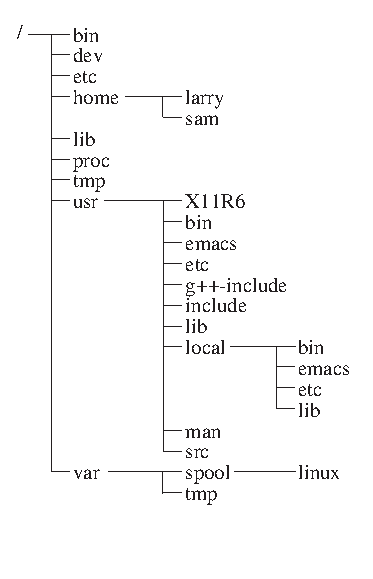
\includegraphics{tutorial/dirtree}}
\label{dirtree}
%\caption{A typical (abridged) {\linux} directory tree.}
\caption{Un t�pico �rbol de directorio {\linux} (resumido).}
\end{figure} } \fi % Kill dirtree if ASCII.

\subsection{Directorio de trabajo actual}
\index{directorio!de trabajo actual!definici�n}
\index{directorio de trabajo!definici�n}
En cualquier momento, se asume que los �rdenes que introduce se refieren a su {\bf directorio de trabajo actual}. Puede entender directorio de trabajo como el directorio en el que ''se encuentra'' 
en ese momento. Cuando accede por primera vez al sistema, su directorio de trabajo se configura como su directorio de usuario ---{\tt /home/larry}, en nuestro caso. Cuando haga referencia a un fichero,
puede referirse a �l en relaci�n a su directorio de trabajo actual, en vez de especificar el nombre de la ruta completa del fichero.

Aqu� tenemos un ejemplo. Larry tiene el directorio {\tt papers}, y {\tt papers} contiene el fichero {\tt history-final}. Si Larry quiere ver el contenido de este fichero, puede usar la orden

\begin{tscreen}
/home/larry\# more /home/larry/papers/history-final
\end{tscreen}

La orden {\tt more} simplemente muestra por pantalla un fichero, pantalla a pantalla. Como el directorio de trabajo actual de Larry es {\tt /home/larry}, se puede referir al fichero {\em en relaci�n\/} con su localizaci�n actual usando la orden

\begin{tscreen}
/home/larry\# more papers/history-final
\end{tscreen}

\index{ruta!relativa}
Si comienza el nombre del fichero (como {\tt papers/final}) con un car�cter diferente de {\tt /}, se est� refiriendo al fichero en t�rminos relativos a su directorio de trabajo actual. Esto se conoce como {\bf nombre de ruta relativo}.

\index{ruta!completa}
\index{ruta!absoluta}
Por otra parte, si comienza el nombre del fichero con una {\tt /}, el sistema lo interpreta como el nombre de la ruta absoluta ---es decir, un nombre de ruta que incluye la ruta completa hasta el fichero, comenzando en el directorio ra�z, {\tt /}. Esto se conoce como {\bf nombre de ruta absoluta}.

\subsection{Refiri�ndose al directorio inicial}
\index{directorio!inicial!\~ para referirse a@{\tt \~{}} para referise a}
\index{\~@{\tt \~{}}!para referirse al directorio inicial}
\index{home}
\index{directorio inicial}
\index{tilde}
\index{virgulilla}
Bajo {\tt tcsh} y {\tt bash}\footnote {{\tt tcsh} y {\tt bash} son dos {\em int�rprete de �rdeness} que funcionan bajo {\linux}. 
El int�rprete de �rdenes es un programa que lee los �rdenes del usuario y los ejecuta; la mayor�a de los sistema {\linux} habilitan 
{\tt tcsh} o {\tt bash} para las cuentas de los nuevos usuarios.}
puede especificar su directorio de usuario con el car�cter de la virgulilla\NT{tilde en ingl�s} ({\tt \~{}}). Por ejemplo, la orden

\begin{tscreen}
/home/larry\# more \~{}/papers/history-final
\end{tscreen}

es equivalente a

\begin{tscreen}
/home/larry\# more /home/larry/papers/history-final
\end{tscreen}

El int�rprete de �rdenes reemplaza el car�cter {\tt \~{}} por el nombre de su directorio de trabajo. 

Puede especificar tambi�n los directorios de usuario de otros usuarios con el car�cter virgulilla. La ruta {\tt \~{}karl/letters} es expandido
a {\tt /home/karl/letters} por el int�rprete de �rdenes (si {\tt /home/karl} es el directorio de usuario de Karl). El uso de la virgulilla es simplemente un atajo; no existe ning�n directorio llamado {\tt \~{}}---es s�lo una ayuda proporcionada por el int�rprete de �rdenes.

\index{{\linux}!conceptos b�sicos|)}

% Linux Installation and Getting Started    -*- TeX -*-
% basic.tex
% Copyright (c) 1992, 1993 by Matt Welsh, Larry Greenfield and Karl Fogel
%
% This file is freely redistributable, but you must preserve this copyright 
% notice on all copies, and it must be distributed only as part of "Linux 
% Installation and Getting Started". This file's use is covered by
% the copyright for the entire document, in the file "copyright.tex".
%
% Copyright (c) 1998 by Specialized Systems Consultants Inc. 
% <ligs@ssc.com>
%Revision 1 realizada el 9 de julio de 2002 por Fco. Javier Fernandez <serrador@arrakis.es>
%Revisi�n 2 Realizada el 17 de julio 2002 por Francisco Javier Fern�ndez <serrador@arrakis.es>

%\section{First steps into Linux.}
\section{Primeros Pasos en {\linux}}
\markboth{Tutorial {\linux }}{Primeros pasos en {\linux}}
Antes de que empecemos, es importante saber que todos 
los nombres de ficheros y �rdenes en un sistema {\linux} 
son {\bf case-sensitive} (que diferencian entre 
may�sculas y min�sculas a diferencia de sistemas 
operativos como MS-DOS). Por ejemplo, la orden {\tt make} 
es muy diferente de {\tt Make} o {\tt MAKE}. Lo mismo se 
cumple para nombres de ficheros y directorios.


\subsection{Movi�ndonos por la estructura de directorios.}
%\subsection{Moving around.}
Ahora que puede entrar en el sistema y que sabe c�mo referenciar los ficheros usando las rutas de los mismos, �c�mo puede cambiar el directorio de trabajo actual, para hacer la vida m�s f�cil?

\index{directorio!estructura!movi�ndose por ella con cd@movi�ndose por ella con cd {\tt cd}}
\index{cd@{\tt cd}|(}
La orden para moverse por la estructura de directorios es {\tt cd}, que es una abreviatura de ''cambiar directorio''.
Muchas de las �rdenes m�s usadas en {\linux} son de dos o tres letras.
La forma de usar la orden {\tt cd} es

\begin{tscreen}
cd \cparam{directorio}
\end{tscreen}

donde  \textsl{directorio} es el nombre del directorio que quiere que se convierta en el directorio de trabajo actual. 

Como se mencion� antes, cuando entra en el sistema, comienza en su directorio de usuario. Si Larry quisiera cambiar al subdirectorio {\tt papers}, usar�a la orden

\begin{tscreen}
/home/larry\# cd papers \\
/home/larry/papers\#
\end{tscreen}

Como puede ver, el indicador de Larry cambia para reflejar 
su directorio de trabajo actual (de forma que sabe d�nde 
se encuentra). Ahora que est� en el directorio  {\tt papers}, 
puede ver history-final con la orden

\begin{tscreen}
/home/larry/papers\# more history-final
\end{tscreen}

\index{directorio!padre!.. para referirse al@{\tt ..} para referirse al}
\index{directorio!. para referirse al@{\tt .} para referirse al}
\index{directorio padre!.. para referirse a@{\tt ..} para referirse a}

Ahora, Larry est� atascado en el subdirectorio {\tt papers}. Para regresar al directorio superior (o padre), ejecute la orden 

\begin{tscreen}
/home/larry/papers\# cd \ .. \\
/home/larry\#
\end{tscreen}

(Observe los espacios entre ``{\tt cd}'' y ``{\tt ..}''.)
Cada directorio tiene una entrada llamada ``{\tt ..}'' que se refiere al directorio padre. De forma similar, cada directorio tiene una entrada llamada ``{\tt .}''que se refiere a s� mismo. Por tanto, la orden 

\begin{tscreen}
/home/larry/papers\# cd \ .
\end{tscreen}

no lleva a ninguna parte. 

Con la orden {\tt cd} se pueden usar tambi�n rutas absolutas.
Para  cambiar  al directorio de usuario de Karl, se puede usar la orden

\begin{tscreen}
/home/larry/papers\# cd /home/karl \\
/home/karl\#
\end{tscreen}

Adem�s, la orden {\tt cd} sin argumentos le llevar� a su propio directorio de usuario. 

\begin{tscreen}
/home/karl\# cd \\
/home/larry\#
\end{tscreen}

\index{cd@{\tt cd}|)}
%\subsection{Looking at the contents of directories.}
\subsection{Mirando el contenido de los directorios}
\label{sec-ls}
\index{directorio!listar los contenidos de|(}
\index{ls@{\tt ls}|(}
\index{listando los contenidos de(}
\index{ficheros!listado|(}

Ahora que sabe c�mo moverse por los directorios, podr�a pensar, �y qu�?. Dar vueltas por los directorios no tiene mucho sentido por s� mismo, as� que introduzcamos una orden nueva,
 {\tt ls}. La orden {\tt ls} muestra un listado de ficheros y directorios, por omisi�n del directorio actual. Por ejemplo:

\begin{tscreen}
/home/larry\# ls \\
Mail \\
letters \\
papers \\
/home/larry\#
\end{tscreen}

Aqu� podemos darnos cuenta de que Larry tiene tres entradas en su directorio actual:  {\tt Mail}, {\tt letters}, y {\tt papers}. Esto no nos dice mucho -- ?` qu� son, directorios o ficheros? 
Podemos usar la opci�n {\tt -F} de la orden {\tt ls} para obtener informaci�n m�s detallada.

\begin{tscreen}
/home/larry\# ls\ --F \\
Mail/ \\
letters/ \\
papers/ \\
/home/larry\#
\end{tscreen}


Por la {\tt /} que aparece en cada nombre, sabemos que estas tres entradas son, de hecho, subdirectorios.

\index{ejecutable!definici�n}
\index{fichero!ejecutable!definici�n}

Ejecutando {\tt ls -F} puede tambi�n aparecer un ``{\tt *}'' al final de un nombre en la lista resultante, lo que indicar�a que el fichero es un {\bf ejecutable} o un programa que puede ejecutarse. 
Si no aparece nada al final de un nombre al usar {\tt ls -F}, el fichero es un ``plain old file'', es decir, no es ni un directorio ni un ejecutable.  

En general, cada orden UNIX puede tomar un cierto n�mero de opciones adem�s de otros argumentos. Estas opciones normalmente comienzan con un ``{\tt -}'', como se vi� arriba con la opci�n {\tt -F}.
 La opci�n {\tt -F} le dice a  {\tt ls} que d� m�s informaci�n acerca del tipo de ficheros involucrados --en nuestro caso, imprimiendo una {\tt /} despu�s de cada nombre de directorio. 

Si le da a {\tt ls} el nombre de un directorio, el sistema listar� los contenidos de ese directorio. 

\begin{tscreen}
/home/larry\# ls\ --F papers \\
english-lit \\
history-final \\
masters-thesis \\
notes/ \\
/home/larry\#
\end{tscreen}

O, para un listado m�s interesante, veamos qu� hay en el directorio de sistema {\tt /etc}. 

\begin{tscreen}
/home/larry\# ls /etc 
\begin{verbatim}
Images          ftpusers        lpc             rc.new          shells
adm             getty           magic           rc0.d           startcons
bcheckrc        gettydefs       motd            rc1.d           swapoff
brc             group           mount           rc2.d           swapon
brc~            inet            mtab            rc3.d           syslog.conf
csh.cshrc       init            mtools          rc4.d           syslog.pid
csh.login       init.d          pac             rc5.d           syslogd.reload
default         initrunlvl      passwd          rmt             termcap
disktab         inittab         printcap        rpc             umount
fdprm           inittab.old     profile         rpcinfo         update
fstab           issue           psdatabase      securetty       utmp
ftpaccess       lilo            rc              services        wtmp
/home/larry#
\end{verbatim}\end{tscreen}

Si es un usuario de MS-DOS, puede que se d� cuenta de que los nombres de ficheros pueden ser mayores de 8 caracteres, y pueden contener puntos en cualquier posici�n. 
Puede incluso usar m�s de un punto en un nombre de fichero.

Vayamos a la parte superior del �rbol de directorios, y luego bajemos a otro directorio con las �rdenes

\begin{tscreen}
/home/larry\# cd .. \\
/home\# cd .. \\
/\# cd usr \\
/usr\# cd bin \\
/usr/bin\#
\end{tscreen}

Puede tambi�n moverse a los directorio en un s�lo paso, haciendo {\tt cd /usr/bin}.

Pruebe a moverse por varios directorios, usando {\tt ls} y {\tt cd}. 
En algunos casos, puede que le aparezca el mensaje de error ``{\tt Permission denied}''\NT{Permiso denegado}. Esto es debido simplemente ``al sistema de seguridad UNIX'':
para poder usar las �rdenes {\tt ls} o {\tt cd}, debe tener permisos para hacerlo. Hablaremos m�s acerca de esto en
 \index{directorio!listado de los contenidos de|)}
 \index{ls@{\tt ls}|)}
 \index{listando los contenidos del directorio|)}
 \index{ficheros!listado|)}
la pagina~\pageref{sec-file-perms}.

%\subsection{Creating new directories.}
\subsection{Creaci�n de directorios nuevos}

\index{directorio!creaci�n}
\index{mkdir@{\tt mkdir}}
Es hora de aprender c�mo crear directorios. Esto requiere el uso de la orden {\tt mkdir}. Pruebe lo siguiente:

\begin{tscreen}
/home/larry\# mkdir foo \\
/home/larry\# ls -F \\
Mail/ \\
foo/ \\
letters/ \\
papers/ \\
/home/larry\# cd foo \\
/home/larry/foo\# ls \\
/home/larry/foo\# 
\end{tscreen}

!`Felicidades! Ha creado un nuevo directorio y se ha metido en �l. Como no hay 
ficheros en este nuevo directorio, aprendamos c�mo copiar ficheros de un lugar a otro.

%\subsection{Copying files.}
\subsection{Copiando ficheros}

\index{ficheros!copiar}
\index{copiar ficheros}
\index{cp@{\tt cp}}

Para copiar ficheros, use el orden {\tt cp}, como se muestra aqu�:

\begin{tscreen}
/home/larry/foo\# cp /etc/termcap\ \ . \\
/home/larry/foo\# cp /etc/shells\ \ . \\
/home/larry/foo\# ls\ --F \\
shells\ \ \ \ \ termcap  \\
/home/larry/foo\# cp shells bells \\
/home/larry/foo\# ls\ --F \\
bells\ \ \ \ \ shells\ \ \ \ \ termcap \\
/home/larry/foo\# 
\end{tscreen}

La orden {\tt cp} copia los ficheros escritos en la l�nea de �rdenes al fichero o directorio dados como �ltimo argumento. D�se cuenta de que usamos``{\tt .}'' para referirnos al directorio 
actual.

%\subsection{Moving files.}
\subsection{Moviendo ficheros}
\index{fichero!mover}
\index{mover ficheros}
\index{mv@{\tt mv}}

El orden {\tt mv} mueve ficheros, en vez de copiarlos. 
La sintaxis es muy parecida:

\begin{tscreen}
/home/larry/foo\# mv termcap sells \\
/home/larry/foo\# ls -F \\
bells\ \ \ \ \ sells\ \ \ \ \ shells \\
/home/larry/foo\# 
\end{tscreen}

D�se cuenta de que el fichero {\tt termcap} ha sido renombrado a {\tt shells}. Puede adem�s usar la orden {\tt mv} para mover un fichero a un directorio completamente 
nuevo.

\blackdiamond {\bf Nota:} {\tt mv} y {\tt cp} sobreescribir�n un fichero de destino que tiene el mismo nombre sin pregunt�rselo. Tenga cuidado cuando mueva un fichero a otro directorio. Puede que haya un fichero con el mismo nombre en ese directorio, !`que ser� sobreescrito!

%\subsection{Deleting ficheros and directories.}
\subsection{Borrando ficheros y directorios}
\index{fichero!borrar}
\index{borrar!ficheros}
\index{rm@{\tt rm}}
Usted tiene ahora una fea rima, que ha creado usando el orden {\tt ls}.
Para borrar un fichero, use el orden {\tt rm}, que proviene de ''remove'',\NT{quitar} como se muestra aqu�:

\begin{tscreen}
/home/larry/foo\# rm bells sells \\
/home/larry/foo\# ls -F \\
shells \\
/home/larry/foo\#
\end{tscreen}

No nos queda nada salvo shells, pero no nos quejaremos. D�se cuenta de que {\tt rm} no 
le preguntar� antes de borrar un fichero, as� que tenga cuidado.

\index{borrar!directorio}
\index{directorio!borrar}
\index{rmdir@{\tt rmdir}}
Una orden relacionada con {\tt rm} es {\tt rmdir}. Este orden borra un directorio, pero s�lo si 
el directorio est� vac�o. Si el directorio contiene alg�n fichero o 
subdirectorio, {\tt rmdir} protestar�.

%\subsection{Looking at ficheros.}
\subsection{Mirando en los ficheros}
\index{ficheros!ver el contenido de}
\index{more@{\tt more}}
\index{cat@{\tt cat}!para ver el contenido de un fichero}
Las �rdenes {\tt more} y {\tt cat} se usan para ver el contenido de los ficheros. El orden {\tt more} muestra un fichero, una pantalla completa cada vez, mientras que {\tt cat} muestra el fichero completo de una vez.

Para ver el contenido del fichero {\tt shells}, use la orden

\begin{tscreen}
/home/larry/foo\# more shells
\end{tscreen}

En caso de que est� interesado en lo que contiene {\tt shells}, es una lista de int�rpretes de �rdenes (shell) v�lidos en su sistema. En la mayor�a de los sistemas, esto incluye {\tt /bin/sh}, {\tt /bin/bash} y {\tt /bin/csh}. Hablaremos acerca de estos diferentes tipos de int�rpretes de �rdenes m�s adelante.

Mientras est� usando {\tt more}, presione \key{Space} para ver la siguiente p�gina de texto, y \key{b} para ver la p�gina anterior. Hay otras �rdenes disponibles en {\tt more},
�stos son s�lo los b�sicos. Podr� salir de {\tt more} pulsando \key{q}.

Salga de {\tt more} y pruebe {\tt cat /etc/termcap}. Probablemente el texto ir� demasiado r�pido para que pueda leerlo. 
El nombre ``{\tt cat}'' proviene de hecho de ``concatenate'', que es el verdadero uso del programa. El orden {\tt cat} puede usarse para "encadenar" los contenidos de varios ficheros y guardar el
 resultado en otro fichero.
Volveremos a esto en la secci�n ~\ref{sec-shell-script}.

%\subsection{Getting online help.}
\subsection{Obteniendo ayuda en l�nea}


\index{{\linux}!p�ginas de manual para}
\index{ayuda!en l�nea}
\index{p�ginas del manual}
\index{maunal de linux}
Casi todos los sistemas UNIX, incluyendo {\linux}, facilitan lo que se conoce como {\bf p�ginas del manual}. Estas p�ginas contienen documentaci�n acerca de �rdenes del sistema, recursos, ficheros
 de configuraci�n, etc.

\index{man@{\tt man}}

La orden usada para acceder a las p�ginas del manual es {\tt man}. Si est� interesado en aprender nuevas opciones de la orden {\tt ls} puede escribir

\begin{tscreen}
/home/larry\# man ls
\end{tscreen}

y se mostrar� la p�gina del manual para {\tt ls}.

Por desgracia, la mayor�a de las p�ginas de manual est�n escritas por personas que ya tienen alguna idea de lo que la orden o recurso hace. Por esta raz�n, las p�ginas del manual, a menudo,
 contienen s�lo los detalles t�cnicos de la orden, sin mucha explicaci�n. De todos modos, las p�ginas del manual pueden constituir un recurso muy valioso para refrescar su memoria si se le 
olvida la sintaxis de una orden. Las p�ginas del manual le hablar�n adem�s de �rdenes que no veremos en este libro.

Sugiero que pruebe {\tt man} para las �rdenes que ya hemos visto y cuando
veamos alguno nuevo. Algunas de estas �rdenes no tendr�n p�gina de manual,
por distintas razones. Primero, las p�ginas de manual puede que no se hayan
escrito todav�a. El proyecto de documentaci�n de {\linux} tambi�n es responsable de
las p�ginas de manual de {\linux}. Estamos acumulando poco a poco la
mayor�a de las p�ginas de manual disponibles para el sistema). Segundo, la
orden podr�a ser una orden interna del shell, o un alias (que se
discutir� en la p�gina ~\pageref{sec-shells-cmds}), la cual podr�a no tener
una p�gina de manual propia. Un ejemplo es {\tt cd}, que es una orden
interna del shell. El shell por s� s�lo procesa la orden {\tt cd} --- 
no hay un programa separado que implemente esta orden.

% {\linux} Installation and Getting Started    -*- TeX -*-
% msdos.tex
% Copyright (c) 1992, 1993 by Matt Welsh <mdw@sunsite.unc.edu>
%
% This file is freely redistributable, but you must preserve this copyright 
% notice on all copies, and it must be distributed only as part of "{\linux} 
% Installation and Getting Started". This file's use is covered by the 
% copyright for the entire document, in the file "copyright.tex".
%
% Copyright (c) 1998 by Specialized Systems Consultants Inc. 
% <ligs@ssc.com>

%\section{Accessing MS-DOS files.}
\section{Acceder a los ficheros MS-DOS\TM}
\markboth{Caracter�sticas Avanzadas}{Acceso a ficheros MS-DOS\tm}
\label{sec-msdos-mount}
\index{MS-DOS!acceder ficheros desde}
\index{ficheros!MS-DOS}
Si, por cualquier retorcida y extrafalaria raz�n, quiere acceder a ficheros
de MS-DOS, lo  podr� hacer f�cilmente desde {\linux}.

\index{MS-DOS!montando una partici�n bajo {\linux}}
\index{mount@{\tt mount}!para montar una partici�n MS-DOS}
La manera normal de acceder a los ficheros de MS-DOS es montar una partici�n MS-DOS o
un disco flexible bajo {\linux}, lo cual permite acceder a los ficheros directamente a trav�s
del sistema de ficheros. Por ejemplo, si tiene un disco flexible MS-DOS en
{\tt /dev/fd0}, la orden

\begin{tscreen}
\# mount -t msdos /dev/fd0 /mnt
\end{tscreen}

lo montar� en {\tt /mnt}. Consulte la Secci�n~\ref{sec-floppy} para m�s
informaci�n sobre c�mo montar discos flexibles.

Tambi�n puede montar una partici�n MS-DOS de su disco duro para que sea
accesible desde {\linux}. Si tiene una partici�n MS-DOS en {\tt /dev/hda1}, la orden

\begin{tscreen}
\# mount -t msdos /dev/hda1 /mnt
\end{tscreen}

la monta. Aseg�rese de desmontar ({\tt umount}) la partici�n cuando haya terminado
de usarla. Tambi�n se puede hacer que una partici�n MS-DOS se monte autom�ticamente
en el momento del arranque si incluye la entrada en {\tt /etc/fstab}. Consulte la
Secci�n~\ref{sec-manage-fs} para m�s detalles. La siguiente l�nea en {\tt
/etc/fstab} monta una partici�n MS-DOS en {\tt /dev/hda1} en el
directorio {\tt /dos}.

\begin{tscreen}
/dev/hda1\ \ \ \ \ /dos\ \ \ \ \ msdos \ \ \ \ \ defaults
\end{tscreen}

Tambi�n puede montar los sistemas de ficheros VFAT usados por Windows 95 y 98:

\begin{tscreen}
\# mount -t vfat /dev/hda1 /mnt
\end{tscreen}

Esto permite acceder a los nombres largos de ficheros de Windows 95\tm. Esto s�lo
se aplica a particiones que realmente tengan almacenados los nombres en formato
largo. No se puede montar un sistema de ficheros FAT16 normal y usarlo para
obtener nombres de ficheros largos.

\index{MS-DOS!uso de Mtools para acceder a ficheros}
El software Mtools tambi�n puede ser usado para acceder a ficheros MS-DOS\tm. Las
�rdenes {\tt mcd}, {\tt mdir}, y {\tt mcopy} se comportan todas como sus
equivalentes MS-DOS\tm. Si instala las Mtools, deber�a tener p�ginas del manual
disponibles para estas �rdenes.

\index{MS-DOS!ejecuci�n de programas bajo {\linux}}
\index{MS-DOS!emulador}
\index{Microsoft Windows!emulador} 
Acceder a ficheros MS-DOS es una cosa; ejecutar programas MS-DOS es
otra. Hay un emulador de MS-DOS\tm en desarrollo para {\linux}; es
f�cil de conseguir, y est� inclu�do en la mayor�a de las distribuciones.
Tambi�n se puede conseguir en muchos sitios, incluyendo los sitios
FTP para {\linux} listados en el Ap�ndice~\ref{app-ftp}. El emulador de MS-DOS est�
considerado como lo suficientemente potente para hacer funcionar un buen n�mero de
aplicaciones, incluyendo Wordperfect\tm, desde {\linux}. Sin embargo, {\linux} y MS-DOS son
sistemas operativos marcadamente diferentes. La potencia de cualquier emulador de MS-DOS
bajo UNIX est� limitada. Adem�s, est� en desarrollo un emulador de Microsoft Windows
que corra bajo X Window.











% \linux Installation and Getting Started    -*- TeX -*-
% commands.tex
% Copyright (c) 1992, 1993 by Matt Welsh, Larry Greenfield and Karl Fogel
%
% This fichero is freely redistributable, but you must preserve this copyright 
% notice on all copies, and it must be distributed only as part of "\linux 
% Installation and Getting Started". This fichero's use is covered by
% the copyright for the entire document, in the fichero "copyright.tex".
%
% Copyright (c) 1998 by Specialized Systems Consultants Inc. 
% <ligs@ssc.com>
% Revisi�n 1 por Fco. Javer Fern�ndez <serrador@arrakis.es> 9 de julio del 2002
%
%\section{Summary of basic UNIX commands.}\label{sec-command-summ}
\section{Sumario de �rdenes b�sicas}
\label{sec-command-summ}
\markboth{Tutorial de {\linux}}{Sumario de �rdenes b�sicas UNIX}

\index{�rdenes!sumario de b�sicas|(}
Esta secci�n introduce algunas de las m�s �tiles �rdenes b�sicas de un sistema UNIX, incluyendo aqu�llas que son cubiertas en la secci�n anterior.

\index{�rdenes!-@{\tt -} flag de opci�n de orden}
\index{flag@{\tt -} de opci�n de orden}
F�jese en que las opciones suelen empezar con ``{\tt -}'', y en la mayor�a de los casos es posible especificar m�s de una opci�n con un �nico ``{\tt -}''. Por ejemplo, en vez de usar {\tt ls -l -F}, 
se puede escribir {\tt ls -lF}.

En lugar de dar una lista de cada una de las opciones de una orden, ahora s�lo vamos a presentar �rdenes �tiles o importantes. De hecho, la mayor�a de estas �rdenes tienen muchas opciones 
que nunca usar�. Puede usar {\tt man} para echar un vistazo a las p�ginas de manual de cada orden, el cu�l lista todas las opciones disponibles.

D�se cuenta tambi�n de que muchas de estas �rdenes toman como argumento una lista de ficheros o directorios, indicados en esta tabla por ``\textsl{fichero1} \ldots \textsl{ficheroN}''. Por ejemplo,
la orden {\tt cp} toma como argumentos una lista de ficheros para copiar, seguido del fichero o directorio destino. Cuando va a copiar m�s de un fichero, el destino debe ser un directorio.

\begin{dispitems}

\index{cd@{\tt cd}}
\ditem {{\tt cd}}
Cambia el directorio de trabajo actual \\
Sintaxis: {\tt cd \cparam{directorio}} \\
Donde \textsl{directorio} es el directorio al que se quiere cambiar. ``{\tt .}''
hace referencia al directorio actual, ``{\tt ..}'' al directorio padre. Si no se especifica ning�n directorio le lleva, por omisi�n, a su directorio de usuario. \\

Ejemplo: {\tt cd ../foo} sube el directorio actual un nivel, y entonces, se introduce en el directorio {\tt foo}.

\index{ls@{\tt ls}}
\ditem {{\tt ls}}
Muestra informaci�n acerca de los ficheros y directorios nombrados. \\
Sintaxis: {\tt ls \cparam{ficheros} }\\
Donde \textsl{ficheros} consiste en los nombres de ficheros o directorios que se quieren listar. Las opciones que m�s se usan son {\tt -F} (para mostrar el tipo de fichero) y {\tt -l}
 (para mostrar una lista ''ampliada'' incluyendo el tama�o de los ficheros, propietario, permisos, etc.). \\
Ejemplo: {\tt ls -lF /home/larry} muestra los contenidos del directorio {\tt /home/larry}.

\index{cp@{\tt cp}}
\ditem {{\tt cp}} 
Copia uno o m�s ficheros a otro fichero o directorio. \\
Sintaxis: {\tt cp \cparam{ficheros}
\cparam{destino}} \\
Donde \textsl{ficheros} indica los ficheros que hay que copiar, y
\textsl{destino} es el fichero o directorio destino. \\

Ejemplo: {\tt cp ../frog joe} copia el fichero {\tt ../frog} al fichero o directorio {\tt joe}.

\index{mv@{\tt mv}}
\ditem {{\tt mv}} 
Mueve uno o m�s ficheros a otro directorio. Esta orden hace el equivalente de una copia seguido del borrado del fichero original.
Puede usar esto para renombrar ficheros, como con la orden de MS-DOS {\tt RENAME}. \\
Sintaxis: {\tt mv \cparam{ficheros}
\cparam{destino}} \\
Donde \textsl{ficheros} indica los arhivos que hay que mover, y
\textsl{destino} es el fichero o directorio destino. \\

Ejemplo: {\tt mv ../frog joe} mueve el fichero {\tt ../frog} al fichero o directorio {\tt joe}.

\index{rm@{\tt rm}}
\ditem {{\tt rm}} 
Borra ficheros. F�jese en que cuando borra un fichero bajo UNIX, 
son irrecuperables (al contrario que con MS-DOS, donde normalmente se puede ''desborrar'' el fichero). \\
Sintaxis: {\tt rm \cparam{ficheros}} \\
Donde \textsl{ficheros} describe el nombre de los ficheros que hay que borrar. \\
La opci�n {\tt -i} le pide confirmaci�n antes de borrar el fichero. \\

Ejemplo: {\tt rm -i /home/larry/joe /home/larry/frog} borra los ficheros {\tt joe} y {\tt frog} en {\tt /home/larry}.


\index{mkdir@{\tt mkdir}}
\ditem {{\tt mkdir}}
Crea nuevos directorios.\\
Sintaxis: {\tt mkdir \cparam{dirs} }\\
Donde \textsl{dirs} son los directorios que hay que crear. \\

Ejemplo: {\tt mkdir /home/larry/test} crea el directorio {\tt test}
en {\tt /home/larry}.

\index{rmdir@{\tt rmdir}}
\ditem {{\tt rmdir}} 
Borra directorios vac�os. Cuando use {\tt rmdir}, el directorio de trabajo actual no debe estar dentro del directorio que se pretende borrar. \\
Sintaxis: {\tt rmdir \cparam{dirs} }\\
Donde \textsl{dirs} define los directorios que hay que borrar. \\

Ejemplo: {\tt rmdir /home/larry/papers} borra el directorio {\tt /home/larry/papers}, si est� vac�o. 

\index{man@{\tt man}}
\ditem {{\tt man}} 
Muestra la p�gina de manual para la orden o recurso dado (es decir, no una utilidad del sistema que no sea 
una orden, como una funci�n de biblioteca.)\\

Sintaxis: {\tt man \cparam{command}} \\

Donde \textsl{command} es el nombre de la orden o recurso del que se quiere conseguir ayuda.\\

Ejemplo: {\tt man ls} le da informaci�n acerca de la orden {\tt ls}.

\index{more@{\tt more}}
\ditem {{\tt more}} 
Muestra informaci�n del contenido de los ficheros nombrados, pantalla por pantalla. \\
Sintaxis: {\tt more \cparam{ficheros}} \\
Donde \textsl{ficheros} indica los ficheros que se quieren mostrar. \\

Ejemplo: {\tt more papers/history-final} muestra el fichero {\tt papers/history-final}.

\index{cat@{\tt cat}}
\ditem {{\tt cat}} 
Oficialmente usado para concatenar ficheros, {\tt cat} tambi�n se usa para mostrar los contenidos de un fichero por pantalla. \\
Sintaxis: {\tt cat \cparam{ficheros}} \\
Donde \textsl{ficheros} indica los ficheros que se quieren mostrar. \\

Ejemplo: {\tt cat letters/from-mdw} muestra el fichero {\tt letters/from-mdw}.

\index{echo@{\tt echo}}
\ditem{{\tt echo}}
Muestra en la pantalla los argumentos que se le pasan a la orden. \\
Sintaxis: {\tt echo \cparam{args}} \\
Donde \textsl{args} indica los argumentos que se quieren mostrar. \\

Ejemplo: {\tt echo ``Hello world''} muestra la cadena ``{\tt Hello world}''.

\index{grep@{\tt grep}}
\ditem{{\tt grep}}
Muestra cada l�nea en uno o m�s ficheros que contiene un patr�n dado. \\
Sintaxis: {\tt grep \cparam{pattern} \cparam{ficheros}} \\
Donde \textsl{pattern} es un patr�n, y 
\textsl{ficheros} indica los ficheros donde se quiere buscar dicho patr�n. \\

Ejemplo: {\tt grep loomer /etc/hosts} muestra cada l�nea en el fichero {\tt /etc/hosts} que contiene el patr�n ``{\tt loomer}''.

\end{dispitems}

\index{�rdenes!sumario de las b�sicas|)}




\chapter{El sistema de archivos}
\label{filesystem-chapter}

\ChapterDescription{Este capitulo describe c�mo el kernel de Linux
  gestiona los ficheros en los sistemas de ficheros soportados por
  �ste.  Describe el Sistema de Ficheros Virtual (VFS) y explica c�mo
  los sistemas de ficheros reales del kernel de Linux son soportados.}

\index{File system} Una de los rasgos m�s importantes de Linux es su
soporte para diferentes sistemas de ficheros.  �sto lo hace muy
flexible y bien capacitado para coexistir con muchos otros sistemas
operativos.  En el momento de escribir �sto, Linux soporta 15 sistemas
de ficheros; \texttt{ext}, \texttt{ext2}, \texttt{xia},
\texttt{minix}, \texttt{umsdos}, \texttt{msdos}, \texttt{vfat},
\texttt{proc}, \texttt{smb}, \texttt{ncp}, \texttt{iso9660},
\texttt{sysv}, \texttt{hpfs}, \texttt{affs} and \texttt{ufs}, y sin
duda, con el tiempo se a�adir�n m�s.

En Linux, como en Unix\tm, a los distintos sistemas de ficheros que el
sistema puede usar no se accede por identificadores de dispositivo
(como un n�mero o nombre de unidad) pero, en cambio se combinan en una
simple structura jer�rquica de �rbol que representa el sistema de
ficheros como una entidad �nica y sencilla.  Linux a�ade cada sistema
de ficheros nuevo en este simple �rbol de sistemas de ficheros cuando
se monta.  Todos los sistemas de ficheros, de cualquier tipo, se
montan sobre un directorio y los ficheros del sistema de ficheros son
el contenido de ese directorio.  Este directorio se conoce como
directorio de montaje o punto de montaje.  Cuando el sistema de
ficheros se desmonta, los ficheros propios del directorio de montaje
son visibles de nuevo.

Cuando se inicializan los discos (usando \eg{fdisk}, por ejemplo)
tienen una estructura de partici�n inpuesta que divide el disco f�sico
en un n�mero de particiones l�gicas.  Cada partici�n puede mantener un
sistema de ficheros, por ejemplo un sistema de ficheros \texttt{EXT2}.
Los sistemas de ficheros organizan los ficheros en structuras
jer�rquicas l�gicas con directorios, enlaces flexibles y m�s
contenidos en los bloques de los dispositivos f�sicos.  Los
dispositivos que pueden contener sistemas de ficheros se conocen con
el nombre de dispositivos de bloque.  La partici�n de disco IDE
\fn{/dev/hda1}, la primera partici�n de la primera unidad de disco en
el sistema, es un dispositivo de bloque.  Los sistemas de ficheros de
Linux contemplan estos dispositivos de bloque como simples colecciones
lineales de bloques, ellos no saben o tienen en cuenta la geometr�a
del disco f�sico que hay debajo.  Es la tarea de cada controlador de
dispositivo de bloque asignar una petici�n de leer un bloque
particular de su dispositivo en t�rminos comprensibles para su
dispositivo; la pista en cuesti�n, sector y cilindro de su disco duro
donde se guarda el bloque.  Un sistema de ficheros tiene que mirar,
sentir y operar de la misma forma sin importarle con que dispositivo
est� tratando.  Por otra parte, al usar los sistemas de ficheros de
Linux, no importa (al menos para el usuario del sistema) que estos
distintos sistemas de ficheros est�n en diferentes soportes
controlados por diferentes controladores de hardware.  El sistema de
ficheros puede incluso no estar en el sistema local, puede ser
perfectamente un disco remoto montado sobre un enlace de red.
Considerese el siguiente ejemplo donde un sistema Linux tiene su
sistema de ficheros ra�z en un disco SCSI:
\begin{verbatim}
A         E         boot      etc       lib       opt       tmp       usr
C         F         cdrom     fd        proc      root      var       sbin
D         bin       dev       home      mnt       lost+found
\end{verbatim}
Ni los usuarios ni los programas que operan con los ficheros necesitan
saber que \fn{/C} de hecho es un sistema de ficheros VFAT montado que
est� en el primer disco IDE del sistema.  En el ejemplo (que es mi
sistema Linux en casa), \fn{/E} es el disco IDE primario en la segunda
controladora IDE.  No importa que la primera controladora IDE sea una
controladora PCI y que la segunda sea una controladora ISA que tambi�n
controla el IDE CDROM.  Puedo conectarme a la red donde trabajo usando
un modem y el protocolo de red PPP y en este caso puedo remotamente
montar mis sistemas de ficheros Linux \axp\ sobre \fn{/mnt/remote}.

Los ficheros en un sistema de ficheros son grupos de datos; el fichero
que contiene las fuentes de este cap�tulo es un fichero ASCII llamado
\fn{filesystems.tex}.  Un sistema de ficheros no s�lo posee los datos
contenidos dentro de los ficheros del sistema de ficheros, adem�s
mantiene la estructura del sistema de ficheros.  Mantiene toda la
informaci�n que los usuarios de Linux y procesos ven como ficheros,
directorios, enlaces flexibles, informaci�n de protecci�n de ficheros
y as�.  Por otro lado debe mantener esa informaci�n de forma eficiente
y segura, la integridad b�sica del sistema operativo depende de su
sistema de ficheros.  Nadie usaria un sistema operativo que perdiera
datos y ficheros de forma aleatoria\footnote{Bueno, no con
  conocimiento, sin embargo me he topado con sistemas operativos con
  m�s abogados que programadores tiene Linux}.

\texttt{Minix}, el primer sistema de ficheros que Linux tuvo es
bastante restrictivo y no era muy r�pido.  \texttt{Minix}, the first
file system that Linux had is rather restrictive and lacking in
performance.\index{Minix} Sus nombres de ficheros no pueden tener m�s
de 14 caracteres (que es mejor que nombres de ficheros 8.3) y el
tama�o m�ximo de ficheros es 64 MBytes.  64 MBytes puede a primera
vista ser suficiente pero se necesitan tama�os de ficheros m�s grandes
para soportar incluso modestas bases de datos.  El primer sistema de
ficheros dise�ado especificamente para Linux, el sistema de Ficheros
Extendido, o \texttt{EXT}, fue introducido en Abril de 1992 y solvent�
muchos problemas pero era aun falto de rapidez.  \index{EXT}
\index{Extended File system} As�, en 1993, el Segundo sistema de
Ficheros Extendido, o \texttt{EXT2}, fue a�adido.  \index{EXT2}
\index{Second Extended File system} Este es el sistema de ficheros que
se describe en detalle m�s tarde en este cap�tulo.

Un importante desarrollo tuvo lugar cuando se a�adi� en sistema de
ficheros EXT en Linux.  El sistema de ficheros real se separ� del
sistema operativo y servicios del sistema a favor de un interfaz
conocido como el sistema de Ficheros Virtual, o VFS.  \index{VFS}
\index{Virtual File system} VFS permite a Linux soportar muchos,
incluso muy diferentes, sistemas de ficheros, cada uno presentando un
interfaz software com�n al VFS.  Todos los detalles del sistema de
ficheros de Linux son traducidos mediante software de forma que todo
el sistema de ficheros parece id�ntico al resto del kernel de Linux y
a los programas que se ejecutan en el sistema.  La capa del sistema de
Ficheros Virtual de Linux permite al usuario montar de forma
transparente diferentes sistemas de ficheros al mismo tiempo.

El sistema de Ficheros Virtual est� implementado de forma que el
acceso a los ficheros es r�pida y tan eficiente como es posible.
Tambi�n debe asegurar que los ficheros y los datos que contiene son
correctos.  Estos dos requisitos pueden ser incompatibles uno con el
otro.  El VFS de Linux mantiene una antememoria con informaci�n de
cada sistema de ficheros montado y en uso.  Se debe tener mucho
cuidado al actualizar correctamente el sistema de ficheros ya que los
datos contenidos en las antememorias se modifican cuando cuando se
crean, escriben y borran ficheros y directorios.  Si se pudieran ver
las estructuras de datos del sistema de ficheros dentro del kernel en
ejecuci�n, se podria ver los bloques de datos que se leen y escriben
por el sistema de ficheros.  Las estructuras de datos, que describen
los ficheros y directorios que son accedidos serian creadas y
destruidas y todo el tiempo los controladores de los dispositivo
estarian trabajando, buascando y guardando datos.  La antememoria o
cach� m�s importantes es el Buffer Cache, que est� integrado entre
cada sistema de ficheros y su dispositivo de bloque.  Tal y como se
accede a los bloques se ponen en el Buffer Cache y se almacenan en
varias colas dependiendo de sus estados.  El Buffer Cache no s�lo
mantiene buffers de datos, tambien ayuda a administrar el interfaz
as�ncrono con los controladores de dispositivos de bloque.

\section{The Second Extended File system (EXT2)}
\index{EXT2}
\begin{figure}
\begin{center}
{\centering \includegraphics{fs/ext2.eps} \par}
\end{center}
\caption{Physical Layout of the EXT2 File system}
\label{ext2fs-figure}
\end{figure}
El Segundo sistema de ficheros Extendido fue pensado (por R�my Card)
como un sistema de ficheros extensible y poderoso para Linux.  Tambi�n
es el sistema de ficheros m�s �xito tiene en la comunidad Linux y es
b�sico para todas las distribuciones actuales de Linux.
\SeeModule{fs/�ext2/�*} El sistema de ficheros EXT2, como muchos
sistemas de ficheros, se construye con la premisa de que los datos
contenidos en los ficheros se guarden en bloques de datos.  Estos
bloques de datos son todos de la misma longitud y, si bien esa
longitud puede variar entre diferentes sistemas de ficheros EXT2 el
tama�o de los bloques de un sistema de ficheros EXT2 en particular se
decide cuando se crea (usando \eg{mke2fs}).  El tama�o de cada fichero
se redondea hasta un numero entero de bloques.  Si el tama�o de bloque
es 1024 bytes, entonces un fichero de 1025 bytes ocupar� dos bloques
de 1024 bytes.  Desafortunadamente esto significa que en promedio se
desperdicia un bloque por fichero.
Normalmente en ordenadores se cambia la carga de CPU por m�s espacio de memoria o de disco utilizado. En este caso Linux, como muchos sistemas operativos, cambia una ineficiencia relativa en el uso del disco a cambio de reducir la carga de la CPU.

No todos los bloques del sistema de ficheros contienen datos, algunos
deben usarse para mantener la informaci�n que describe la estructura
del sistema de ficheros.  EXT2 define la topologia del sistema de
ficheros describiendo cada fichero del sistema con una estructura de
datos inodo.  Un inodo describe que bloques ocupan los datos de un
fichero y tambi�n los permisos de acceso del fichero, las horas de
modificaci�n del fichero y el tipo del fichero.  Cada fichero en el
sistema de ficheros EXT2 se describe por un �nico inodo y cada inodo
tiene un �nico n�mero que lo identifica.  Los inodos del sistema de
ficheros se almacenan juntos en tablas de inodos.  Los directorios
EXT2 son simplemente ficheros especiales (ellos mismos descritos por
inodos) que contienen punteros a los inodos de sus entradas de
directorio.

La figura�\ref{ext2fs-figure} muestra la disposici�n del sistema de
ficheros EXT2 ocupando una serie de bloques en un dispositivo
estructurado bloque.  Por la parte que le toca a cada sistema de
ficheros, los dispositivos de bloque son s�lo una serie de bloques que
se pueden leer y escribir.  Un sistema de ficheros no se debe
preocupar donde se debe poner un bloque en el medio f�sico, eso es
trabajo del controlador del dispositivo.  Siempre que un sistema de
ficheros necesita leer informaci�n o datos del dispositivo de bloque
que los contiene, pide que su controlador de dispositivo lea un n�mero
entero de bloques.  El sistema de ficheros EXT2 divide las particiones
l�gicas que ocupa en Grupos de Bloque (Block Groups).  \index{EXT2
  Block Groups} Cada grupo duplica informaci�n cr�tica para la
integridad del sistema de ficheros ya sea valiendose de ficheros y
directorios como de bloques de informaci�n y datos.  Esta duplicaci�n
es necesaria por si ocurriera un desastre y el sistema de ficheros
necesitara recuperarse.  Los subapartados describen con m�s detalle
los contenidos de cada Grupo de Bloque.

\subsection{El inodo de EXT2}
\begin{figure}
\begin{center}
{\centering \includegraphics{fs/ext2_inode.eps} \par}
\end{center}
\caption{El inodo de EXT2}
\label{ext2fs-inode-figure}
\end{figure}
\index{El inodo de EXT2} \index{Estructuras de datos, el inodo EXT2} En el sistema de ficheros \texttt{EXT2}, el inodo es el bloque de construcci�n
b�sico; cada fichero y directorio del sistema de ficheros es descrito
por un y s�lo un inodo.  Los inodos EXT2 para cada Grupo de Bloque se
almacenan juntos en la table de inodos con un mapa de bits que permite
al sistema seguir la pista de inodos reservados y libres.  La
figura�\ref{ext2fs-inode-figure} muestra el formato de un inodo EXT2,
entre otra informaci�n, contiene los siguientes campos:
\SeeModule{include/\-linux/\-ext2\_fs\_i.h}
\begin{description}
\item [mode] Esto mantiene dos partes de informaci�n; qu� inodo
  describe y los permisos que tienen los usuarios.  Para EXT2, un
  inodo puede describir un ficheros, directorio, enlace simb�lico,
  dispositivo de bloque, dispositivo de caracter o FIFO.
\item [Owner Information] Los identificadores de usuario y grupo de
  los due�os de este fichero o directorio.  Esto permite al sistema de
  ficheros aplicar correctamente el tipo de acceso,
\item [Size] El tama�o en del fichero en bytes,
\item [Timestamps] La hora en la que el inodo fue creado y la �ltima
  hora en que se modific�,
\item [Datablocks] Punteros a los bloques que contienen los datos que
  este inodo describe.  Los doce primeros son punteros a los bloques
  f�sicos que contienen los datos descritos por este inodo y los tres
  �ltimos punteros contienen m�s y m�s niveles de indirecci�n.  Por
  ejemplo, el puntero de doble indirecci�n apunta a un bloque de
  punteros que apuntan a bloques de punteros que apuntan a bloques de
  datos.  Esto significa que ficheros menores o iguales a doce bloques
  de datos en longitud son m�s facilmente accedidos que ficheros m�s
  grandes.
\end{description}
Indicar que los inodos EXT2 pueden describir ficheros de dispositivo
especiales.  No son ficheros reales pero permiten que los programas
puedan usarlos para acceder a los dispositivos.  Todos los ficheros de
dispositivo de \fn{/dev} est�n ahi para permitir a los programas
acceder a los dispositivos de Linux.  Por ejemplo el programa
\eg{mount} toma como argumento el fichero de dispositivo que el
usuario desee montar.

\subsection{El superbloque EXT2}
\index{Superbloque EXT2} El Superbloque contiene una descripci�n del
tama�o y forma base del sistema de ficheros.  La informaci�n contenida
permite al administrador del sistema de ficheros usar y mantener el
sistema de ficheros.  Normalmente s�lo se lee el Superbloque del Grupo
de Bloque 0 cuando se monta el sistema de ficheros pero cada Grupo de
Bloque contiene una copia duplicada en caso de que se corrompa sistema
de ficheros.  Entre otra informaci�n contiene el:
\SeeModule{include/\-linux/\-ext2\_fs\_sb.h}
\begin{description}
\item [Magic Number] Esto permite al software de montaje comprobar que
  es realmente el Superbloque para un sistema de ficheros EXT2.  Para
  la versi�n actual de \texttt{EXT2} �ste es \hex{EF53}.
\item [Revision Level] Los niveles de revisi�n mayor y menor permiten
  al c�digo de montaje determinar si este sistema de ficheros soporta
  o no caracter�sticas que s�lo son disponibles para revisiones
  particulares del sistema de ficheros.  Tambi�n hay campos de
  compatibilidad que ayudan al c�digo de montaje determinar que nuevas
  caracter�sticas se pueden usar con seguridad en ese sistema de
  ficheros,
\item [Mount Count and Maximum Mount Count] Juntos permiten al sistema
  determinar si el sistema de ficheros fue comprobado correctamente.
  El contador de montaje se incrementa cada vez que se monta el
  sistema de ficheros y cuando es igual al contador m�ximo de montaje
  muestra el mensaje de aviso �maximal mount count reached, running
  e2fsck is recommended�,
\item [Block Group Number] El n�mero del Grupo de Bloque que tiene la
  copia de este Superbloque,
\item [Block Size] El tama�{o} de bloque para este sistema deficheros
  en bytes, por ejemplo 1024 bytes,
\item [Blocks per Group] El n�mero de bloques en un grupo.  Como el
  tama�o de bloque �ste se fija cuando se crea el sitema de ficheros,
\item [Free Blocks] EL n�mero de bloques libres en el sistema de
  ficheros,
\item [Free Inodes] El n�mero de Inodos libres en el sistema de
  ficheros,
\item [First Inode] Este es el n�mero de inodo del primer inodo en el
  sistema de ficheros.  El primer inodo en un sistema de ficheros EXT2
  ra�z seria la entrada directorio para el directorio '/'.
\end{description}

\subsection{The EXT2 Group Descriptor}
\index{EXT2 Group Descriptor} Cada Grupo de Bloque tiene una
estructura de datos que lo describe.  Como el Superbloque, todos los
descriptores de grupo para todos los Grupos de Bloque se duplican en
cada Grupo de Bloque en caso de corrupci�n del sistema de fichero.
\SeeCode{ext2\_group\_desc}{include/\-linux/\-ext2\_fs.h} Cada
Descriptor de Grupo contiene la siguiente informaci�n:
\begin{description}
\item [Blocks Bitmap] El n�mero de bloque del mapa de bits de bloques
  reservados para este Grupo de Bloque.  Se usa durante la reseva y
  liberaci�n de bloques,
\item [Inode Bitmap] El n�mero de bloque del mapa de bits de inodos
  reservados para este Grupo de Bloques.  Se usa durante la reserva y
  liberaci�n de inodos,
\item [Inode Table] El n�mero de bloque del bloque inicial para la
  tabla de inodos de este Grupo de Bloque.  Cada inodo se representa
  por la estructura de datos inodo EXT2 descrita abajo.
        \item [Free blocks count, Free Inodes count, Used directory count]
\end{description}
Los descriptores de grupo se colocan uno detr�s de otro y juntos hacen
la tabla de descriptor de grupo.  Cada Grupo de Bloques contiene la
tabla entera de descriptores de grupo despues de su copia del
Superbloque.  S�lo la primera copia (en Grupo de Bloque 0) es usada
por el sistema de ficheros EXT2.  Las otras copias est�n ahi, como las
copias del Superbloque, en caso de que se corrompa la principal.

\subsection{EXT2 Directories}
\index{EXT2 Directories}
\index{Data structures, EXT2 Directory}
\begin{figure}
\begin{center}
{\centering \includegraphics{fs/ext2_dir.eps} \par}
\end{center}
\caption{EXT2 Directory}
\label{ext2fs-dir-figure}
\end{figure}
En el sistema de ficheros EXT2, los directorios son ficheros
especiales que se usan para crear y mantener rutas de acceso a los
ficheros en el sistema de ficheros.  La figura�\ref{ext2fs-dir-figure}
muestra la estructura de una estrada directorio en memoria.
\SeeCode{ext2\_dir\_entry}{include/\-linux/\-ext2\_fs.h} Un fichero
directorio es una lista de entradas directorio, cada una conteniendo
la siguiente informaci�n:
\begin{description}
\item [inode] El inodo para esta entrada directorio.  Es un �ndice al
  vector de inodos guardada en la Tabla de Inodos del Grupo de Bloque.
  En la figura�\ref{ext2fs-dir-figure}, la entrada directorio para el
  fichero llamado \fn{file} tiene una referencia al n�mero de inodo
  \texttt{i1},
\item [name length] La longitud de esta entrada directorio en bytes,
        \item [name] El nombre de esta entrada directorio.
\end{description}
Las dos primeras entradas para cada directorio son siempre las
entradas estandar �.� y �..� significando �este directorio� y �el
directorio padre� respectivamente.

\subsection{Finding a File in an EXT2 File System}
Un nombre de fichero Linux tiene el mismo formato que los nombres de
ficheros de todos los Unix\tm\.  Es una serie de nombres de
directorios separados por contra barras (�\fn{/}�) y acabando con el
nombre del fichero.  Un ejemplo de nombre de fichero podria ser
\fn{/home/rusling/.cshrc} donde \fn{/home} y \fn{/rusling} son nombres
de directorio y el nombre del fichero es \fn{.cshrc}.  Como todos los
demas sistemas Unix\tm� Linux no tiene encuenta el formato del nombre
del fichero; puede ser de cualquier longitud y cualquier caracter
imprimible.  Para encontrar el inodo que representa a este fichero
dentro de un sistema de ficheros \texttt{EXT2} el sistema debe
analizar el nombre del fichero directorio a directorio hasta encontrar
el fichero en si.  El primer inodo que se necesita es el inodo de la
ra�z del sistema de ficheros, que est� en el superbloque del sistema
de ficheros.  Para leer un inodo EXT2 hay que buscarlo en la tabla de
inodos del Grupo de Bloque apropiado.  Si, por ejemplo, el n�mero de
inodo de la ra�z es 42, entonces necesita el inodo 42avo de la tabla
de inodos del Grupo de Bloque 0.  El inodo ra�z es para un directorio
EXT2, en otras palabras el modo del inodo lo describe como un
directorio y sus bloques de datos contienen entradas directorio EXT2.

\fn{home} es una de las muchas entradas directorio y esta entrada
directorio indica el n�mero del inodo que describe al directorio
\fn{/home}.  Hay que leer este directorio (primero leyendo su inodo y
luego las entradas directorio de los bloques de datos descritos por su
inodo) para encontrar la entrada \fn{rusling} que indica el numero del
inodo que describe al directorio \fn{/home/rusling}.  Finalmente se
debe leer las entradas directorio apuntadas por el inodo que describe
al directorio \fn{/home/rusling} para encontrar el n�mero de inodo del
fichero \fn{.cshrc} y desde ahi leer los bloques de datos que
contienen la informaci�n del fichero.

\subsection{Changing the Size of a File in an EXT2 File System}
Un problema com�n de un sistema de ficheros es la tendencia a
fragmentarse.  Los bloques que contienen los datos del fichero se
esparcen por todo el sistema de ficheros y esto hace que los accesos
secuenciales a los bloques de datos de un fichero sean cada vez m�s
ineficientes cuanto m�s alejados est�n los bloques de datos.  El
sistema de ficheros EXT2 intenta solucionar esto reservando los nuevos
bloques para un fichero, fisicamente juntos a sus bloques de datos
actuales o al menos en el mismo Grupo de Bloque que sus bloques de
datos.  S�lo cuando esto falla, reserva bloques de datos en otros
Grupos de Bloque.

Siempre que un proceso intenta escribir datos a un fichero, el sistema
de ficheros Linux comprueba si los datos exceden el final del �ltimo
bloque para el fichero.  Si lo hace, entonces tiene que reservar un
nuevo bloque de datos para el fichero.  Hasta que la reserva no haya
acabado, el proceso no puede ejecutarse; debe esperarse a que el
sistema de ficheros reserve el nuevo bloque de datos y escriba el
resto de los datos antes de continuar.  La primera cosa que hacen las
rutinas de reserva de bloques EXT2 es bloquear el Superbloque EXT2 de
ese sistema de ficheros.  La reserva y liberaci�n cambia campos del
superbloque, y el sistema de ficheros Linux no puede permitir m�s de
un proceso haciendo �sto a la vez.  Si otro proceso necesita reservar
m�s bloques de datos, debe esperarse hasta que el otro proceso acabe.
Los procesos que esperan el superbloque son suspendidos, no se pueden
ejecutar, hasta que el control del superbloque lo abandone su usuario
actual.  El acceso al superbloque se garantiza mediante una pol�tica
�el primero que llega se atiende primero�, y cuando un proceso tiene
control sobre el superbloque le pone cerrojo hasta que no lo necesita
m�s. \footnote{REVISAR!!!} bloqueado el superbloque, el proceso
comprueba que hay suficientes bloques libres en ese sistema de
ficheros.  Si no es as�, el intento de reservar m�s bloques falla y el
proceso ceder� el control del superbloque del sistema de ficheros.

Si hay suficientes bloques en el sistema de ficheros, el proceso
intenta reservar uno.
\SeeCode{ext2\_new\_block()}{fs/\-ext2/\-balloc.c} Si el sistema de
ficheros EXT2 se ha compilado para prereservar bloques de datos
entonces se podr� usar uno de estos.  La prereserva de bloques no
existe realmente, s�lo se reservan dentro del mapa de bits de bloques
reservados.  El inodo VFS que representa el fichero que intenta
reservar un nuevo bloque de datos tiene dos campos EXT2 espec�ficos,
\field{prealloc\_block} y \field{prealloc\_count}, que son el numero
de bloque del primer bloque de datos prereservado y cuantos hay,
respectivamente.  Si no habian bloques prereservados o la reserva
anticipada no est� activa, el sistema de ficheros EXT2 debe reservar
un nuevo bloque.  El sistema de ficheros EXT2 primero mira si el
bloque de datos despues del �ltimo bloque de datos del fichero est�
libre.  Logicamente, este es el bloque m�s eficiente para reservar ya
que hace el acceso secuencial mucho m�s r�pido.  Si este bloque no
est� libre, la b�squeda se ensancha y busca un bloque de datos dentro
de los 64 bloques del bloque ideal.  Este bloque, aunque no sea ideal
est� al menos muy cerca y dentro del mismo Grupo de Bloque que los
otros bloques de datos que pertenecen a ese fichero.

Si incluso ese bloque no est� libre, el proceso empieza a buscar en
los dem�s Grupos de Bloque hasta encontrar algunos bloques libres.  El
c�digo de reserva de bloque busca un cluster de ocho bloques de datos
libres en cualquiera de los Grupos de Bloque.  Si no puede encontrar
ocho juntos, se ajustar� para menos.  Si se quiere la prereserva de
bloques y est� activado, actualizar� \field{prealloc\_block} y
\field{prealloc\_count} pertinentemente.

Donde quiera que encuentre el bloque libre, el c�digo de reserva de
bloque actualiza el mapa de bits de bloque del Grupo de Bloque y
reserva un buffer de datos en el buffer cach�.  Ese buffer de datos se
identifica unequivocamente por el identificador de dispositivo del
sistema y el n�mero de bloque del bloque reservado.  El buffer de
datos se sobreescribe con ceros y se marca como �sucio� para indicar
que su contenido no se ha escrito al disco f�sico.  Finalmente, el
superbloque se marca como �sucio� para indicar que se ha cambiado y
est� desbloqueado.  Si hubiera otros procesos esperando, al primero de
la cola se le permitiria continuar la ejecuci�n y terner el control
exclusido del superbloque para sus operaciones de fichero.  Los datos
del proceso se escriben en el nuevo bloque de datos y, si ese bloque
se llena, se repite el proceso entero y se reserva otro bloque de
datos.

\section{The Virtual File System (VFS)}
\index{Virtual File System (VFS)}
\index{VFS}
\begin{figure}
\begin{center}
{\centering \includegraphics{fs/vfs.eps} \par}
\end{center}
\caption{A Logical Diagram of the Virtual File System}
\label{vfs-figure}
\end{figure}
La figura�\ref{vfs-figure} muestra la relaci�n entre el Sistema de
Ficheros Virtual del kernel de Linux y su sistema de ficheros real.
El sistema de ficheros vitual debe mantener todos los diferentes
sistemas de ficheros que hay montados en cualquier momento.  Para
hacer esto mantiene unas estructuras de datos que describen el sistema
de ficheros (virtual) por entero y el sistema de ficheros, montado,
real.  \SeeModule{fs/*} De forma m�s confusa, el VFS describe los
ficheros del sistema en t�rminos de superbloque e inodos de la misma
forma que los ficheros EXT2 usan superbloques e inodos.  Como los
inodos EXT2, los inodos VFS describen ficheros y directorios dentro
del sistema; los contenidos y topolog�a del Sistema de Ficheros
Virtual.  De ahora en adelante, para evitar confusiones, se escribir�
inodos CFS y superbloques VFS para distinguirlos de los inodos y
superbloques EXT2.

Cuando un sistema de ficheros se inicializa, se registra �l mismo con
el VFS.  Esto ocurre cuando el sistema operativo se inicializa en el
momento de arranque del sistema.  Los sistemas de ficheros reales
est�n compilados con el nucleo o como m�dulos cargables.  Los m�dulos
de Sistemas de Ficheros se cargan cuando el sistema los necesita, as�,
por ejemplo, si el sistema de ficheros \texttt{VFAT} est� implementado
como m�dulo del kernel, entonces s�lo se carga cuando se monta un
sistema de ficheros \texttt{VFAT}.  Cuando un dispositivo de bloque
base se monta, y �ste incluye el sistema de ficheros ra�z, el VFS debe
leer su superbloque.  Cada rutina de lectura de superbloque de cada
tipo de sistema de ficheros debe resolver la topolog�a del sistema de
ficheros y mapear esa informaci�n dentro de la estructura de datos del
superbloque VFS.  El VFA mantiene una lista de los sitema de ficheros
montados del sistema junto con sus superbloques VFS.  Cada superbloque
VFS contiene informaci�n y punteros a rutinas que realizan funciones
particulares.  De esta forma, por ejemplo, el superbloque que
representa un sistema de ficheros EXT2 montado contiene un puntero a
la rutina de lectura de inodos espec�fica.  Esta rutina, como todas
las rutinas de lectura de inodos del sistema de ficheros espe�fico,
rellena los campos de un inodo VFS.  Cada superbloque VFS contiene un
puntero al primer inodo VFS del sistema de ficheros.  Para el sistema
de ficheros ra�z, �ste es el inodo que representa el directorio
\fn{�/�}.  Este mapeo de informaci�n es muy eficiente para el sistema
de ficheros EXT2 pero moderadamente menos para otros sistema de
ficheros.

Ya que los procesos del sistema acceden a directorios y ficheros, las
rutinas del sistema se dice que recorren los inodos VFS del sistema.
\SeeModule{fs/�inode.c} Por ejemplo, escribir \eg{ls} en un directorio
o \eg{cat} para un fichero hacen que el Sistema de Ficheros Virtual
busque atrav�s de los inodos VFS que representan el sistema de
ficheros.  Como cada fichero y directorio del sistema se representa
por un inodo VFS, un n�mero de inodos ser�n accedidos repetidamente.
Estos inodos se mantienen en la antememoria, o cach�, de inodos que
hace el acceso mucho m�s r�pido.  Si un inodo no est� en la cach�,
entonces se llama a una rutina espec�fica del sistema de ficheros para
leer el inodo apropiado.  La acci�n de leer el inodo hace que se ponga
en la cach� de inodos y siguientes accesos hacen que se mantenga en la
cach�.  Los inodos VFS menos usados se quitan de la cach�.

Todos los sistemas de ficheros de Linux usan un buffer cach� com�n
para mantener datos de los dispositivos para ayudar a acelerar el
acceso por todos los sistemas de ficheros al dispositivo f�sico que
contiene los sistemas de ficheros.  \SeeModule{fs/�buffer.c} Este
buffer cach� es independiente del sistema de ficheros y se integra
dentro de los mecanismos que el n�cleo de Linux usa para reservar,
leer y escribir datos.  Esto tiene la ventaja de hacer los sistemas de
ficheros de Linux independientes del medio y de los controladores de
dispositivos que los soportan.  Tofos los dispositivos estructurados
de bloque se registran ellos mismos con el n�cleo de Linux y presentan
una interfaz uniforme, basada en bloque y normalmente as�ncrona.
Incluso dispositivos de bloque relativamente complejos como SCSI lo
hacen.

Cuando el sistema de ficheros real lee datos del disco f�sico realiza
una petici�n al controlador de dispositivo de bloque para leer los
bloques f�sicos del dispositivo que controla.  Integrado en este
interfaz de dispositivo de bloque est� el buffer cach�.  Al leer
bloques del sistema de ficheros se guardan en un el buffer cach�
global compartido por todos los sistemas de ficheros y el n�cleo de
Linux.  Los buffers que hay dentro se identifican por su n�mero de
bloque y un identificador �nico para el dispositivo que lo ha leido.
De este modo, si se necesitan muy a menudo los mismos datos, se
obtendr�n del buffer cach� en lugar de leerlos del disco, que tarda
m�s tiempo.  Algunos dispositivos pueden realizar lecturas anticipadas
(\textit{read ahead}), mediante lo cual se realizan lecturas antes de
necesitarlas, especulando con que se utilizar�n m�s
adelante.\footnote{REVISAR!!!!!} 

El VFS tambi�n mantiene una cach� de directorios donde se pueden
encontrar los inodos de los directorios que se usan de forma m�s
frecuente.  \SeeModule{fs/�dcache.c} Como experimento, probar a listar
un directorio al que no se haya accedido recientemente.  La primera
vez que se lista, se puede notar un peque�o retardo pero la segunda
vez el resultado es inmediato.  El cach� directorio no almacena
realmente los inodos de los directorios; �stos estar�n en el cach� de
inodos, el directorio cach� simplemente almacena el mapa entre el
nombre entero del directorio y sus n�meros de inodo.

\subsection{The VFS Superblock}
\index{Superblock, VFS} \index{VFS superblock} Cada sistema de
ficheros montado est� representado por un superbloque VFS; entre otra
informaci�n, el superbloque VFS contiene:
\SeeModule{include/�linux/�fs.h}
\begin{description}
\item [Device] Es el identificador de dispositivo para el dispositivo
  bloque que contiene este a este sistema de ficheros.  Por ejemplo,
  \fn{/dev/hda1}, el primer disco duro IDE del sistema tiene el
  identificador de dispositivo \hex{301},
\item [Inode pointers] El puntero de inodo \field{montado} apunta al
  primer inodo del sistema de ficheros.  El puntero de inodo
  \field{cubierto} apunta al inodo que representa el directorio donde
  est� montado el sistema de ficheros.  El superbloque VFS del sistema
  de ficheros ra�z no tiene puntero \field{cubierto},
\item [Blocksize] EL tama�o de bloque en bytes del sistema de
  ficheros, por ejemplo 1024 bytes,
\item [Superblock operations] Un puntero a un conjunto de rutinas de
  superbloque para ese sistema de ficheros.  Entre otras cosas, estas
  rutinas las usa el VFS para leer y escribir inodos y superbloques.
\item [File System type] Un puntero a la estructura de datos
  \ds{tipo\_sistema\_ficheros} del sistema de ficheros montado,
\item [File System specific] Un puntero a la informaci�n que necesaria
  este sistema de ficheros.
\end{description}

\subsection{The VFS Inode}
\index{inode, VFS} \index{VFS inode} Como el sistema de ficheros EXT2,
cada fichero, directorio y dem�s en el VFS se representa por uno y
solo un inodos VFS.  \SeeModule{include/�linux/�fs.h} La infomaci�n en
cada inodo VFS se construye a partir de informaci�n del sistema de
ficheros por las rutinas espec�ficas del sistema de ficheros.  Los
inodos VFS existen s�lo en la memoria del n�cleo y se mantienen en el
cach� de inodos VFS tanto tiempo como sean �tiles para el sistema.
Entre otra informaci�n, los inodos VFS contienen los siguientes
campos:
\begin{description}
\item [device] Este es el identificador de dispositivo del dispositivo
  que contiene el fichero o lo que este inodo VFS represente,
\item [inode number] Este es el n�mero del inodo y es �nico en este
  sistema de ficheros.  La combinaci�n de \field{device} y
  \field{inode number} es �nica dentro del Sistema de Ficheros
  Virtual,
\item [mode] Como en EXT2 este campo describe que representa este
  inodo VFS y sus permisos de acceso,
\item [user ids] Los identificadores de propietario,
\item [times] Los tiempos de creaci�n, modificaci�n y escritura,
\item [block size] El tama�o de bloque en bytes para este fichero, por
  ejemplo 1024 bytes,
\item [inode operations] Un puntero a un bloque de direcciones de
  rutina.  Estas rutinas son espef�ficas del sistema de ficheros y
  realizan operaciones para este inodo, por ejemplo, truncar el
  fichero que representa este inodo.
\item [count] El n�mero de componentes del sistema que est�n usando
  actualmente este inodo VFS.  Un contador de cero indica que el inodo
  est� libre para ser descartado o reusado,
\item [lock] Este campo se usa para bloquear el inodo VFS, por
  ejemplo, cuando se lee del sistema de ficheros,
\item [dirty] Indica si se ha escrito en este inodo, si es as�{i} el
  sistema de ficheros necesitar� modificarlo,
\item [file system specific information]
\end{description}

\subsection{Registering the File Systems}
\begin{figure}
\begin{center}
{\centering \includegraphics{fs/file-systems.eps} \par}
\end{center}
\caption{Registered File Systems}
\label{file-systems-figure}
\end{figure}
\index{File System, registering} \index{Registering a file system}
Cuando se compila el n�cleo de Linux se pregunta si se quiere cada uno
de los sistemas de ficheros soportados.  Cuando el n�cleo est�
compilado, el c�difo de arranque del sistema de ficheros contiene
llamadas a las rutinas de inicializaci�n de todos los sistemas de
ficheros compilados.  \SeeCode{sys\_setup()}{fs/\-filesystems.c} Los
sistemas de ficheros de Linux tambi�n se pueden compilar como m�dulos
y, en este caso, pueden ser cargados cuando se les necesita o
cargarlos a mano usando \eg{insmod}.  Siempre que un m�dulo de sistema
de ficheros se carga se registra �l mismo con el n�cleo y se borra �l
mismo cuando se descarga.  Cada rutina de inicializaci�n del sistema
de ficheros se registra con el Sistema de Ficheros Virtual y se
representa por una estructura de datos \ds{tipo\_sistema\_ficheros}
que contiene el nombre del sistema de ficheros y un puntero a su
rutina de lectura de superbloque VFS.  La
figura�\ref{file-systems-figure} muestra que las estructuras de datos
\ds{tipo\_sistems\_ficheros} se ponen en una lista apuntada por el
puntero \ds{sistemas\_ficheros}.  Cada estructura de datos
\ds{tipo\_sistema\_ficheros} contiene la siguiente informaci�n:
\SeeCode{file\_system\_type}{include/\-linux/\-fs.h}
\begin{description}
\item [Superblock read routine] Esta rutina se llama por el VFS cuando
  se monta una instancia del sistema de ficheros,
\item [File System name] El nombre de este sistema de ficheros, por
  ejemplo \texttt{ext2},
\item [Device needed] Necesita soportar este sistema de ficheros un
  dispositivo?  No todos los sistemas de ficheros necesitan un
  dispositivo.  El sistema de fichero \texttt{/proc}, por ejemplo, no
  requiere un dispositivo de bloque,
\end{description}
Se puede ver que sistemas de ficheros hay rgistrados mirando en
\fn{/proc/filesystems}.  Por ejemplo:
\begin{verbatim}
      ext2
nodev proc
      iso9660
\end{verbatim}

\subsection{Mounting a File System}
\index{Mounting a File System} \index{File System, mounting} Cuando el
superusuario intenta montar un sistema de ficheros, el n�cleo de Linux
debe primero validar los argumentos pasados en la llamada al sistema.
Aunque \eg{mount} hace una comprobaci�n b�sica, no conoce que sistemas
de ficheros soporta el kernel o si existe el punto de montaje
propuesto.  Considerar el siguiente comando \eg{mount}:
\begin{verbatim}
$ mount -t iso9660 -o ro /dev/cdrom /mnt/cdrom
\end{verbatim}% $ para que no moleste el modo AUC-TeX de Emacs
Este comando \eg{mount} pasa al n�cleo tres trozos de informaci�n; el
nombre del sistema de ficheros, el dispositivo de bloque f�sico que
contiene al sistema de fichros y, por �ltimo, donde, en la topolog�a
del sistema de ficheros existente, se montar� el nuevo sistema de
ficheros.

La primera cosa que debe hacer el Sistema de Ficheros Virtual es
encontrar el sistema de ficheros.  \SeeCode{do\_mount()}{fs/\-super.c}
Para hacer �{es}to busca a trav�s de la lista de sistemas de ficheros
conocidos y mira cada estructura de datos ds{tipo\_sistema\_ficheros}
en la lista apuntada por \ds{sistema\_ficheros}.
\SeeCode{get\_fs\_type()}{fs/\-super.c} Si encuentra una coincidencia
del nombre ahora sabe que ese tipo de sistema de ficheros es soportado
por el n�cleo y tiene la direcci�n de la rutina espec�fica del sistema
de ficheros para leer el superbloque de ese sistema de ficheros.  Si
no puede encontrar ninguna coindidencia no todo est� perdido si el
n�cleo puede cargar m�dulos por demanda (ver
Cap�tulo�\ref{modules-chapter}).  En este caso el n�cleo piede al
demonio del n�cleo que cargue el m�dulo del sistema de ficheros
apropiado antes de continuar como anteriormente.

Si el dispositivo f�sico pasado por \eg{mount} no est� ya montado,
debe encontrar el inodo VFS del directorio que ser� el punto de
montaje del nuevo sistema de ficheros.  Este inodo VFS debe estar en
el cach� de inodos o se debe leer del dispositivo de bloque que
soporta el sistema de ficheros del punto de montaje.  Una vez que el
inodo se ha encontrado se comprueba para ver que sea un directorio y
que no contenga ya otro sistema de ficheros montado.  El mismo
directorio no se puede usar como punto de montaje para m�s de un
sistema de ficheros.

En este punto el c�difo de montaje VFS reserva un superbloque VFS y le
pasa la informaci�n de montahe a la rutina de lectura de superblque
para este sistema de ficheros.  Todos los superbloques VFS del sistema
se mantienen en el vector \ds{super\_bloques} de las estructuras de
datos \ds{super\_bloque} y se debe reservar una para este montaje.  La
rutina de lectura de superbloque debe rellenar los campos b�sicos del
superbloque VFS con informaci�n que lee del dispositivo f�sico.  Para
el sistema de ficheros EXT2 este mapeo o traducci�n de informaci�n es
bastante facil, simplemente lee el superbloque EXT2 y rellena el
superbloque VFS de ah�.  Para otros sistemas de ficheros, como el MS
DOS, no es una tarea t�n facil.  Cualquiera que sea el sistema de
ficheros, rellenar el superbloque VFS significa que el sistema de
ficheros debe leer todo lo que lo describe del dispositivo de bloque
que lo soporta.  Si el dispositivo de bloque no se puede leer o si no
contiene este tipo de sistema de ficheros entonces el comando
\eg{mount} fallar�.

\begin{figure}
\begin{center}
{\centering \includegraphics{fs/mounted.eps} \par}
\end{center}
\caption{A Mounted File System}
\label{mounted-figure}
\end{figure}
Cada sistema de ficheros montado es descrito por una estructura de
datos \ds{vfsmount}; ver figura�\ref{mounted-figure}.  Estos son
puestos en una cola de una lista apuntada por \ds{vfsmntlist}.
\SeeCode{add\_vfsmnt()}{fs/�super.c} Otro puntero, \ds{vfsmnttail}
apunta a la �ltima entrada de la lista y el puntero
\dsni{mru\_vfsmnt}\index{mru\_vfsmnt pointer} apunta al sistemas de
ficheros m�s recientemente usado.  Cada estructura \ds{vfsmount}
contiene el n�mero de dispositivo del dispositivo de bloque que
contiene al sistema de ficheros, el directorio donde el sistema de
ficheros est� montado y un puntero al superbloque VFS reservado cuando
se mont�.  En cambio el superbloque VFS apunta a la estructura de
datos \ds{tipo\_sistema\_ficheros} para este tipo de sisetma de
ficheros y al inodo ra�{i}z del sistema de ficheros.  Este inodo se
mantiene residente en el cach� de inodos VFS todo el tiempo que el
sistema de ficheros est� cargado.

\subsection{Finding a File in the Virtual File System}
\index{Finding a File} \index{Files, finding} Para encontrar el inodo
VFS de un fichero en el Sistema de Ficheros Virtual, VFS debe resolver
el nombre del directorio, mirando el inodo VFS que representa cada uno
de los directorios intermedios del nombre.  Mirar cada directorio
envuelve una llamada al sistema de ficheros espec�fico cuya direcci�n
se mantiene en el inodo VFS que representa al directorio padre.  Esto
funciona porque siempre tenemos el inodo VFS del ra�z de cada sistema
de ficheros disponible y apuntado por el superbloque VFS de ese
sistema.  Cada vez que el sistema de ficheros real mira un inodo
comprueba el cach� de directorios.  Si no est� la entrada en el cach�
de directorios, el sistema de ficheros real toma el inodo VFS tanto
del sistema de ficheros como del cach� de inodos.

\subsection{Creating a File in the Virtual File System}
\index{Creating a file}
\index{Files, creating}

\subsection{Unmounting a File System}
\index{Unmounting a File System} \index{File System, unmounting} The
workshop manual for my MG usually describes assembly as the reverse of
disassembly and the reverse is more or less true for unmounting a file
system.  \SeeCode{do\_umount()}{fs/�super.c} A file system cannot be
unmounted if something in the system is using one of its files.  So,
for example, you cannot umount \fn{/mnt/cdrom} if a process is using
that directory or any of its children.  If anything is using the file
system to be unmounted there may be VFS inodes from it in the VFS
inode cache, and the code checks for this by looking through the list
of inodes looking for inodes owned by the device that this file system
occupies.  If the VFS superblock for the mounted file system is dirty,
that is it has been modified, then it must be written back to the file
system on disk.  Once it has been written to disk, the memory occupied
by the VFS superblock is returned to the kernel's free pool of memory.
Finally the \ds{vfsmount} data structure for this mount is unlinked
from \ds{vfsmntlist} and freed.
\SeeCode{remove\_vfsmnt()}{fs/�super.c}

\subsection{The VFS Inode Cache}
\index{Inode cache} \index{Caches, VFS inode} As the mounted file
systems are navigated, their VFS inodes are being continually read
and, in some cases, written.  The Virtual File System maintains an
inode cache to speed up accesses to all of the mounted file systems.
Every time a VFS inode is read from the inode cache the system saves
an access to a physical device.  \SeeModule{fs/�inode.c}

The VFS inode cache is implmented as a hash table whose entries are
pointers to lists of VFS inodes that have the same hash value.  The
hash value of an inode is calculated from its inode number and from
the device identifier for the underlying physical device containing
the file system.  Whenever the Virtual File System needs to access an
inode, it first looks in the VFS inode cache.  To find an inode in the
cache, the system first calculates its hash value and then uses it as
an index into the inode hash table.  This gives it a pointer to a list
of inodes with the same hash value.  It then reads each inode in turn
until it finds one with both the same inode number and the same device
identifier as the one that it is searching for.

If it can find the inode in the cache, its count is incremented to
show that it has another user and the file system access continues.
Otherwise a free VFS inode must be found so that the file system can
read the inode from memory.  VFS has a number of choices about how to
get a free inode.  If the system may allocate more VFS inodes then
this is what it does; it allocates kernel pages and breaks them up
into new, free, inodes and puts them into the inode list.  All of the
system's VFS inodes are in a list pointed at by \ds{first\_inode} as
well as in the inode hash table.  If the system already has all of the
inodes that it is allowed to have, it must find an inode that is a
good candidate to be reused.  Good candidates are inodes with a usage
count of zero; this indicates that the system is not currently using
them.  Really important VFS inodes, for example the root inodes of
file systems always have a usage count greater than zero and so are
never candidates for reuse.  Once a candidate for reuse has been
located it is cleaned up.  The VFS inode might be dirty and in this
case it needs to be written back to the file system or it might be
locked and in this case the system must wait for it to be unlocked
before continuing.  The candidate VFS inode must be cleaned up before
it can be reused.

However the new VFS inode is found, a file system specific routine
must be called to fill it out from information read from the
underlying real file system.  Whilst it is being filled out, the new
VFS inode has a usage count of one and is locked so that nothing else
accesses it until it contains valid information.

To get the VFS inode that is actually needed, the file system may need
to access several other inodes.  This happens when you read a
directory; only the inode for the final directory is needed but the
inodes for the intermediate directories must also be read.  As the VFS
inode cache is used and filled up, the less used inodes will be
discarded and the more used inodes will remain in the cache.

\subsection{The Directory Cache}
\index{Directory cache} \index{Caches, directory} To speed up accesses
to commonly used directories, the VFS maintains a cache of directory
entries.  \SeeModule{fs/�dcache.c} As directories are looked up by the
real file systems their details are added into the directory cache.
The next time the same directory is looked up, for example to list it
or open a file within it, then it will be found in the directory
cache.  Only short directory entries (up to 15 characters long) are
cached but this is reasonable as the shorter directory names are the
most commonly used ones.  For example, \fn{/usr/X11R6/bin} is very
commonly accessed when the X server is running.

The directory cache consists of a hash table, each entry of which
points at a list of directory cache entries that have the same hash
value.  The hash function uses the device number of the device holding
the file system and the directory's name to calculate the offset, or
index, into the hash table.  It allows cached directory entries to be
quickly found.  It is no use having a cache when lookups within the
cache take too long to find entries, or even not to find them.

In an effort to keep the caches valid and up to date the VFS keeps
lists of Least Recently Used (LRU) directory cache entries.  When a
directory entry is first put into the cache, which is when it is first
looked up, it is added onto the end of the first level LRU list.  In a
full cache this will displace an existing entry from the front of the
LRU list.  As the directory entry is accessed again it is promoted to
the back of the second LRU cache list.  Again, this may displace a
cached level two directory entry at the front of the level two LRU
cache list.  This displacing of entries at the front of the level one
and level two LRU lists is fine.  The only reason that entries are at
the front of the lists is that they have not been recently accessed.
If they had, they would be nearer the back of the lists.  The entries
in the second level LRU cache list are safer than entries in the level
one LRU cache list.  This is the intention as these entries have not
only been looked up but also they have been repeatedly referenced.

\ReviewNotes{Do we need a diagram for this?}

\section{The Buffer Cache}
\index{Buffer caches}
\index{Caches, buffer}
\begin{figure}
\begin{center}
{\centering \includegraphics{fs/buffer-cache.eps} \par}
\end{center}
\caption{The Buffer Cache}
\label{buffer-cache-figure}
\end{figure}
As the mounted file systems are used they generate a lot of requests
to the block devices to read and write data blocks.  All block data
read and write requests are given to the device drivers in the form of
\ds{buffer\_head} data structures via standard kernel routine calls.
These give all of the information that the block device drivers need;
the device identifier uniquely identifies the device and the block
number tells the driver which block to read.  All block devices are
viewed as linear collections of blocks of the same size.  To speed up
access to the physical block devices, Linux maintains a cache of block
buffers.  All of the block buffers in the system are kept somewhere in
this buffer cache, even the new, unused buffers.  This cache is shared
between all of the physical block devices; at any one time there are
many block buffers in the cache, belonging to any one of the system's
block devices and often in many different states.  If valid data is
available from the buffer cache this saves the system an access to a
physical device.  Any block buffer that has been used to read data
from a block device or to write data to it goes into the buffer cache.
Over time it may be removed from the cache to make way for a more
deserving buffer or it may remain in the cache as it is frequently
accessed.

Block buffers within the cache are uniquely identfied by the owning
device identifier and the block number of the buffer.  The buffer
cache is composed of two functional parts.  The first part is the
lists of free block buffers.  There is one list per supported buffer
size and the system's free block buffers are queued onto these lists
when they are first created or when they have been discarded.  The
currently supported buffer sizes are 512, 1024, 2048, 4096 and 8192
bytes.  The second functional part is the cache itself.  This is a
hash table which is a vector of pointers to chains of buffers that
have the same hash index.  The hash index is generated from the owning
device identifier and the block number of the data block.
Figure�\ref{buffer-cache-figure} shows the hash table together with a
few entries.  Block buffers are either in one of the free lists or
they are in the buffer cache.  When they are in the buffer cache they
are also queued onto Least Recently Used (LRU) lists.  There is an LRU
list for each buffer type and these are used by the system to perform
work on buffers of a type, for example, writing buffers with new data
in them out to disk.  The buffer's type reflects its state and Linux
currently supports the following types:
\begin{description}
\item [clean] Unused, new buffers,
\item [locked] Buffers that are locked, waiting to be written,
\item [dirty] Dirty buffers.  These contain new, valid data, and will
  be written but so far have not been scheduled to write,
\item [shared] Shared buffers,
\item [unshared] Buffers that were once shared but which are now not
  shared,
\end{description}

Whenever a file system needs to read a buffer from its underlying
physical device, it trys to get a block from the buffer cache.  If it
cannot get a buffer from the buffer cache, then it will get a clean
one from the appropriate sized free list and this new buffer will go
into the buffer cache.  If the buffer that it needed is in the buffer
cache, then it may or may not be up to date.  If it is not up to date
or if it is a new block buffer, the file system must request that the
device driver read the appropriate block of data from the disk.

Like all caches, the buffer cache must be maintained so that it runs
efficiently and fairly allocates cache entries between the block
devices using the buffer cache.  Linux uses the \texttt{bdflush}
\index{bdflush, kernel daemon} \index{Kernel daemons, bdflush} kernel
daemon to perform a lot of housekeeping duties on the cache but some
happen automatically as a result of the cache being used.

\subsection{The \texttt{bdflush} Kernel Daemon}
\index{bdflush, kernel daemon} \index{Kernel daemons, bdflush}
\SeeCode{bdflush()}{fs/�buffer.c} The \texttt{bdflush} kernel daemon
is a simple kernel daemon that provides a dynamic response to the
system having too many dirty buffers; buffers that contain data that
must be written out to disk at some time.  It is started as a kernel
thread at system startup time and, rather confusingly, it calls itself
�kflushd� and that is the name that you will see if you use the
\eg{ps} command to show the processes in the system.  Mostly this
daemon sleeps waiting for the number of dirty buffers in the system to
grow too large.  As buffers are allocated and discarded the number of
dirty buffers in the system is checked.  If there are too many as a
percentage of the total number of buffers in the system then
\texttt{bdflush} is woken up.
The default threshold is 60% but, if the system is desperate for buffers, \texttt{bdflush}
will be woken up anyway.
This value can be seen and changed using the \eg{update} command:
\begin{verbatim}

# update -d

bdflush version 1.4
0:    60 Max fraction of LRU list to examine for dirty blocks
1:   500 Max number of dirty blocks to write each time bdflush activated
2:    64 Num of clean buffers to be loaded onto free list by refill_freelist
3:   256 Dirty block threshold for activating bdflush in refill_freelist
4:    15 Percentage of cache to scan for free clusters
5:  3000 Time for data buffers to age before flushing
6:   500 Time for non-data (dir, bitmap, etc) buffers to age before flushing
7:  1884 Time buffer cache load average constant
8:     2 LAV ratio (used to determine threshold for buffer fratricide).

\end{verbatim}
All of the dirty buffers are linked into the \texttt{BUF\_DIRTY} LRU
list whenever they are made dirty by having data written to them and
\texttt{bdflush} tries to write a reasonable number of them out to
their owning disks.  Again this number can be seen and controlled by
the \eg{update} command and the default is 500 (see above).

\subsection{The \eg{update} Process}
\index{update process} The \eg{update} command is more than just a
command; it is also a daemon.  When run as superuser (during system
initialisation) it will periodically flush all of the older dirty
buffers out to disk.  It does this by calling a system service routine
\SeeCode{sys\_bdflush()}{fs/�buffer.c} that does more or less the same
thing as \texttt{bdflush}.  Whenever a dirty buffer is finished with,
it is tagged with the system time that it should be written out to its
owning disk.  Every time that \eg{update} runs it looks at all of the
dirty buffers in the system looking for ones with an expired flush
time.  Every expired buffer is written out to disk.

\section{The /proc File System}
\index{/proc file system} The \texttt{/proc} file system really shows
the power of the Linux Virtual File System.  It does not really exist
(yet another of Linux's conjuring tricks), neither the \texttt{/proc}
directory nor its subdirectories and its files actually exist.  So how
can you \eg{cat} \fn{/proc/devices}?  The {/proc} file system, like a
real file system, registers itself with the Virtual File System.
However, when the VFS makes calls to it requesting inodes as its files
and directories are opened, the \texttt{/proc} file system creates
those files and directories from information within the kernel.  For
example, the kernel's \fn{/proc/devices} file is generated from the
kernel's data structures describing its devices.

The \texttt{/proc} file system presents a user readable window into
the kernel's inner workings.  Several Linux subsystems, such as Linux
kernel modules described in chapter�\ref{modules-chapter}, create
entries in the the \texttt{/proc} file system.

\section{Ficheros especiales de dispostivo}
\index{Device Special Files} Linux, like all versions of Unix\tm\ 
presents its hardware devices as special files.  So, for example,
/dev/null is the null device.  A device file does not use any data
space in the file system, it is only an access point to the device
driver.  The EXT2 file system and the Linux VFS both implement device
files as special types of inode.  There are two types of device file;
character and block special files.  Within the kernel itself, the
device drivers implement file semantices: you can open them, close
them and so on.  Character devices allow I/O operations in character
mode and block devices require that all I/O is via the buffer cache.
When an I/O request is made to a device file, it is forwarded to the
appropriate device driver within the system.  Often this is not a real
device driver but a pseudo-device driver for some subsystem such as
the SCSI device driver layer.  Device files are referenced by a major
number, which identifies the device type, and a minor type, which
identifies the unit, or instance of that major type.  For example, the
IDE disks on the first IDE controller in the system have a major
number of 3 and the first partition of an IDE disk would have a minor
number of 1.  So, \texttt{ls -l}\index{ls command} of \fn{/dev/hda1}
gives: \marginnote{see \fn{/include/linux/\\major.h} for all of
  Linux's major device numbers.}
\begin{verbatim}
$ brw-rw----   1 root    disk       3,    1  Nov 24  15:09 /dev/hda1
\end{verbatim}
Within the kernel, every device is uniquely described by a
\dsni{kdev\_t}\index{kdev\_t data type} data type, this is two bytes
long, the first byte containing the minor device number and the second
byte holding the major device number.
\SeeModule{include/�linux/�kdev\_t.h} The IDE device above is held
within the kernel as \hex{0301}.  An EXT2 inode that represents a
block or character device keeps the device's major and minor numbers
in its first direct block pointer.  When it is read by the VFS, the
VFS inode data structure representing it has its \field{i\_rdev} field
set to the correct device identifier.

% \linux: Instalaci�n y primeros pasos      -*- TeX -*-
% shells.tex
% Copyright (c) 1992, 1993 by Matt Welsh, Larry Greenfield and Karl Fogel
%
% Este fichero puede redistribuirse libremente, pero debe conservarse este distintivo 
% de copyright en todas las copias, y s�lo debe ser distribuido como parte de 
% "\linux: Instalaci�n y primeros pasos". El uso de este archvi est� cubierto por el 
% copyright para todo el documento, en el arhcivo "copyright.tex"
%
% Copyright (c) 1998 by Specialized Systems Consultants Inc. 
% <ligs@ssc.com>
%\section{Types of shells.}
%Revisado por Francisco javier Fern�ndez el 17 de julio de 2002

\section{Tipos de int�rpretes de �rdenes}
\markboth{Tutorial de {\linux}}{Las Shells o int�rpretes de �rdenes} 
 \index{shells|(}

Como se ha comentado antes, {\linux} es un sistema operativo multitarea y multiusuario.
La multitarea es {\em muy} �til, y una vez la haya comprendido, la usar� todo el
tiempo. Dentro de poco ejecutar� programas en segundo plano, cambiar� entre tareas
y redirigir� programas junto a resultados complicados con una sencilla orden.

Muchas de las caracter�sticas que se ver�n en esta secci�n son caracter�sticas
suministradas por el int�rprete de �rdenes. Se debe tener cuidado en no confundir
{\linux} (el actual sistema operativo) con el int�rprete de �rdenes. 
Un int�rprete de �rdenes es tan s�lo un interfaz con el sistema operativo que hay 
debajo. El int�rprete de �rdenes proporciona funcionalidad a�adida a {\linux}.

\index{shell scripts!definici�n}
Un int�rprete de �rdenes no es s�lo un int�rprete de las �rdenes interactivas que
se teclean en el indicador de �rdenes, sino tambi�n un potente lenguaje de programaci�n. Permite
escribir {\bf guiones (shell scripts)}, juntando varias �rdenes en un fichero. Si se conoce
MS-DOS, se reconocer� la similitud con los ficheros de procesamiento por lotes. Los
guiones del int�rprete de �rdenes son una herramienta muy potente, que le
permitir� automatizar y extender el uso de {\linux}. Mire la p�gina~\pageref{sec-shell-script} para m�s informaci�n.

\index{shells!Bourne shell}
\index{shells!C shell}
\index{Bourne shell}
\index{C Shell (csh)@C Shell ({\tt csh})}
\index{/bin/sh@{\tt /bin/sh}}
\index{/bin/csh@{\tt /bin/csh}}

Hay varios tipos de int�rprete de �rdenes \NT{{\em shell}, escudo en ingl�s} en el mundo de Unix.
Los m�s importantes son la ``{\em shell Bourne}'' y la ``{\em shell C}''. La 
{\em shell Bourne} utiliza una sintaxis de �rdenes como la {\em shell} original de 
los primeros sistemas UNIX, como System III. El nombre de la {\em shell Bourne} en 
la mayor�a de los sistemas {\linux} es {\tt /bin/sh} (donde {\tt sh} significa ``{\em 
shell}''. La {\em shell C} (no confundir con una concha marina) utiliza diferente 
sintaxis, parecida al lenguaje de programaci�n ``C'', y en la mayor�a de los 
sistemas {\linux} se llama {\tt/bin/csh}.

\index{shells!Bourne again shell}
\index{Bourne again shell}
\index{bash@{\tt bash}}
\index{/bin/bash@{\tt /bin/bash}}
\index{Tcsh}
\index{/bin/tcsh@{\tt /bin/tcsh}}
\index{tcsh@{\tt tcsh}}


Bajo {\linux}, hay disponibles muchas variaciones de int�rpretes de �rdenes. Las
dos m�s com�nmente utilizadas son {\em Bourne Again Shell}, o ``bash'' ({\tt/bin/bash}),
y ``Tcsh'' ({\tt /bin/tcsh}). La variante {\tt bash} es una forma de {\em shell Bourne} que incluye
muchas de las caracter�sticas avanzadas de la {\em shell C}. A causa de que {\tt bash}
soporta un superconjunto de sintaxis de la {\em shell Bourne}, los {\em guiones} de la 
{\em shell} escritos en el est�ndar de la shell Bourne podr�an trabajar con {\tt 
bash}. Si se prefiere la sintaxis de la {\em shell C}, {\linux} soporta {\tt tcsh}, 
que es una versi�n ampliada de la {\em shell C}.

El tipo de {\em shell} que usted decida utilizar ser� sobre todo una cuesti�n de fe. 
Algunas personas prefieren la sintaxis de la {\em shell Bourne} con las 
caracter�sticas avanzadas de {\tt bash}, y otros prefieren la sintaxis m�s estructurada 
de la {\em shell C}. Por lo que respecta a �rdenes normales como {\tt cp} y {\tt ls}, la
{\em shell} que se use no importa, la sintaxis es la misma. S�lo cuando se 
comienzan a escribir {\em guiones de �rdenes} o a usar las caracter�sticas avanzadas de
la {\em shell}, comienzan a importar las diferencias entre los tipos de {\em shell}.
Al discutir las caracter�sticas de varios int�rpretes, se notar�n las diferencias
entre las {\em shells} C y Bourne. Sin embargo, para los prop�sitos de este manual,
la mayor�a de estas diferencias son m�nimas (si realmente est�s interesado en
este punto, lea las p�ginas sobre {\tt bash} y {\tt tcsh}).\NT{Tambi�n puede leer
el ``Bash Scripting HOWTO''}
\index{shells|)}




% Linux: Instalaci�n y Primeros Pasos    -*- TeX -*-
% wildcard.tex
% Copyright (c) 1992, 1993 by Matt Welsh, Larry Greenfield and Karl Fogel
%
% Este archivo puede redistribuirse libremente, pero debe conservarse este distintivo 
% de copyright en todas las copias, y s�lo debe ser distribuido como parte de 
% "Linux: Instalaci�n y primeros pasos". El uso de este archvi est� cubierto por el 
% copyright para todo el documento, en el arhcivo "copyright.tex"
%
% Copyright (c) 1998 by Specialized Systems Consultants Inc. 
% <ligs@ssc.com>
% Revisi�n 1 por Francisco javier Fern�ndez 31 de agosto de 2002
%\section{Wildcards.}
\section{Caracteres comod�n}
\markboth{Tutorial de {\linux}}{Comodines}

\index{shells!caracteres comod�n para|(}
\index{caracteres comodin!en nombres de fichero|(}
\index{nombres de fichero!caracteres comod�n en|(}
\index{caracteres comod�nes!definici�n}
Una caracter�stica importante de la mayor�a de sistemas {\linux} es la 
posibilidad de referirse a m�s de un fichero usando caracteres especiales. 
Estos {\bf caracteres comod�n} le permiten referirse a todos los nombres de 
fichero que contengan el car�cter ``{\tt n}''.

\index{*@{\tt *}}
\index{caracteres comod�n!*@{\tt *}}
El comod�n `{\tt *}'' especifica cualquier car�cter o cadena de caracteres 
en el nombre de un fichero. Cuando usa el car�cter  ``{\tt *}'' en un
nombre de fichero, el int�rprete de �rdenes lo reemplaza con todas las posibles 
sustituciones de los nombres de fichero en el directorio al que est� 
haciendo referencia.

He aqu� un r�pido ejemplo. Suponga que Larry tiene los ficheros {\tt frog},
{\tt joe} y {\tt stuff} en su directorio actual.
\begin{tscreen}
/home/larry\# ls \\
frog\ \ \ \ \ joe\ \ \ \ \ stuff \\
/home/larry\#
\end{tscreen}

Para especificar todos los ficheros que contienen la letra ``o'' en el
nombre de fichero, use la instrucci�n
\begin{tscreen}
/home/larry\# ls *o* \\
frog\ \ \ \ \ joe \\
/home/larry\#
\end{tscreen}
Como puede ver, cada instancia de ``{\tt *}'' es reemplazada con todas
las sustituciones que coinciden con los nombres de fichero del directorio
actual.

El uso de ``{\tt *}'' s�lo, simplemente coincide con todos los nombres de 
fichero, porque todos los caracteres coinciden con el comod�n.
\begin{tscreen}
/home/larry\# ls * \\
frog\ \ \ \ \ joe\ \ \ \ \ stuff \\
/home/larry\#
\end{tscreen}

Aqu� hay algunos ejemplos m�s:
\begin{tscreen}
/home/larry\# ls f* \\
frog \\
/home/larry\# ls *ff \\
stuff \\
/home/larry\# ls *f* \\
frog\ \ \ \ \ stuff \\
/home/larry\# ls s*f \\
stuff \\
/home/larry\# 
\end{tscreen}

\index{expansion de comodines!definicion}
\index{shells!expansi�n de comodines}
El proceso de cambiar un ``{\tt *}'' en una serie de nombres de fichero se llama
{\bf expansi�n de comodines} y lo hace el int�rprete de �rdenes. Esto es importante: 
una orden individual, como {\tt ls}, {\em nunca} ve el ``{\tt *}'' en su lista de 
par�metros. El int�rprete de �rdenes expande el comod�n para incluir todos los
nombres de fichero que coinciden. As�, la orden
\begin{tscreen}
/home/larry\# ls *o*
\end{tscreen}
es expandido por el int�rprete de �rdenes a 
\begin{tscreen}
/home/larry\# ls frog joe
\end{tscreen}

\index{ficheros!ocultos!no hacen juego con los comodines}
Una nota importante del comod�n ``{\tt *}'' : {\em no} ve las coincidencias
de los nombres de fichero que empiezan con un �nico punto (``{\tt .}'').  
Estos ficheros se tratan como ficheros {\bf ocultos} --- aunque no est�n 
realmente escondidos, no aparecen en los listados normales con {\tt ls} y 
no son afectados por el uso del comod�n ``{\tt *}''.

He aqu� un ejemplo. Mencionamos antes que cada directorio  contiene dos 
entradas especiales: ``{\tt .}'' se refiere al directorio actual, y
``{\tt ..}'' , que se refiere al directorio padre. Sin embargo, cuando usa 
{\tt ls}, estas dos entradas no se muestran.
\begin{tscreen}
/home/larry\#  ls \\
frog\ \ \ \ \ joe\ \ \ \ \ stuff \\
/home/larry\# 
\end{tscreen}
Si usa el par�metro {\tt -a} con {\tt ls}, sin embargo, puede visualizar
los nombres de fichero que empiezan con ``{\tt .}''. Observe:
\begin{tscreen}
/home/larry\# ls -a \\
.\ \ \ \ \ ..\ \ \ \ \ .bash\_profile\ \ \ \ \ .bashrc\ \ \ \ \ frog
\ \ \ \ \ joe\ \ \ \ \ stuff \\
/home/larry\# 
\end{tscreen}
El listado contiene las dos entradas especiales, ``{\tt .}'' y ``{\tt
..}'', as� como otros dos ficheros ``ocultos'' --{\tt .bash\_profile}
y {\tt .bashrc}--. Estos dos ficheros son ficheros de inicio usados por
{\tt bash} cuando {\tt larry} entra en el sistema. Se describen en 
p�gina~\pageref{sec-init-scripts}.

Hay que fijarse en que cuando usa el comod�n ``{\tt *}'' , ninguno de los 
nombres de fichero que empiezan por ``{\tt .}'' son visualizados.
\begin{tscreen}
/home/larry\# ls * \\
frog\ \ \ \ \ joe\ \ \ \ \ stuff \\
/home/larry\# 
\end{tscreen}
Esto es una caracter�stica de seguridad: si el comod�n ``{\tt *}'' tiene 
coincidencias con nombres de fichero que empiezen por ``{\tt .}'', tambi�n 
tendr�a coincidencia con los nombres de directorios ``{\tt .}'' y 
``{\tt ..}''. Esto puede ser peligroso al usar ciertas �rdenes.

\index{caracteres comod�n!?@{\tt ?}}
\index{?@{\tt ?}}
Otro comod�n es ``{\tt ?}''.  El comod�n ``{\tt ?}'' s�lo se expande 
a un car�cter. As�, ``{\tt ls ?}'' muestra todos los nombres 
de fichero de un s�lo car�cter. Y ``{\tt ls termca?}'' mostrar�a 
``{\tt termcap}'' pero {\em no\/} ``{\tt termcap.backup}''.  Aqu� 
hay otros ejemplos:
\begin{tscreen}
/home/larry\# ls j?e \\
joe \\
/home/larry\# ls f??g \\
frog \\
/home/larry\# ls ????f \\
stuff \\
/home/larry\# 
\end{tscreen}

Como puede ver, los comodines le permiten especificar muchos ficheros 
a la vez. En el sumario de �rdenes que empieza en la p�gina~\pageref{sec-command-summ}, 
dijimos que las �rdenes {\tt cp} y {\tt mv} realmente pueden copiar o mover m�s 
de un fichero a la vez. Por ejemplo,
\begin{tscreen}
/home/larry\# cp /etc/s* /home/larry
\end{tscreen}
copia todos los ficheros de {\tt /etc} cuyo nombre empieza por ``{\tt s}'' al 
directorio {\tt /home/larry}. El formato de la orden {\tt cp} es realmente
\begin{tscreen}
cp \cparam{ficheros}   \cparam{destino}
\end{tscreen}
donde \textsl{ficheros} lista los nombres de fichero a copiar, y \textsl{destino} 
es el fichero o directorio destino.
La orden {\tt mv} tiene una sintaxis id�ntica.

Si est� copiando o moviendo m�s de un fichero, el \textsl{destino} tiene
que ser un directorio. S�lo puede copiar o mover un �nico fichero a otro fichero.

\index{shells!caracteres comod�n para|)}
\index{caracteres comod�n!en nombres de fichero|)}
\index{nombres de fichero!caracteres comod�n en|)}

% \linux: Instalaci�n y primeros pasos    -*- TeX -*-
% plumbing.tex
% Copyright (c) 1992, 1993 by Matt Welsh, Larry Greenfield and Karl Fogel
%
% Este fichero puede redistribuirse libremente, pero debe conservarse este distintivo 
% de copyright en todas las copias, y s�lo debe ser distribuido como parte de 
% "\linux: Instalaci�n y primeros pasos". El uso de este archvi est� cubierto por el 
% copyright para todo el documento, en el fichero "copyright.tex".
%
% Copyright (c) 1998 by Specialized Systems Consultants Inc. 
% <ligs@ssc.com>
%Revisi�n 1 por Francisco Javier Fern�ndez
%Revisi�n 2 por Fco. J Fern�ndez  el 9 de septiembre de 2002
%\section{\linux plumbing.} \label{sec-plumbing}
\section{Fontaner�a \linux} 
\label{sec-plumbing}
\markboth{Tutorial de  {\linux} }{Fontaner�a {\linux}}

%\subsection{Standard input and standard output.}
\subsection{Entrada y salida est�ndar.}
\index{standard input|(}
\index{standard output|(}
\index{stdin}
\index{stdout}
\index{entrada est�ndar}
\index{salida est�ndar}

Muchas instrucciones de {\linux} toman la entrada de lo que se llama {\bf standard input}
y mandan su salida a  {\bf standard output} (a menudo abreviados como
{\tt stdin} y {\tt stdout}). El int�rprete de �rdenes arregla las cosas de forma que la entrada
est�ndar es su teclado y la salida est�ndar es la pantalla.

He aqu� un ejemplo en el que se usa la orden {\tt cat}. Normalmente, 
{\tt cat} lee datos de todos los argumentos especificados por la l�nea de 
�rdenes y manda estos datos directamente a {\tt stdout}. Por tanto 
usando la orden 
\begin{tscreen}
/home/larry/papers\# cat history-final masters-thesis
\end{tscreen}
se muestra el contenido del fichero {\tt history-final} seguido por 
{\tt masters-thesis}. 

Sin embargo, si no especifica un nombre de fichero, {\tt cat} lee datos 
de {\tt stdin} y los devuelve a {\tt stdout}. Aqu� hay un ejemplo:
\begin{tscreen}
/home/larry/papers\# cat \\
Hello there. \\
Hello there. \\
Bye. \\
Bye. \\
\key{Ctrl-D} \\
/home/larry/papers\# 
\end{tscreen}
\index{se�al de fin-de-texto}
\index{EOT!se�al}
Cada l�nea que escriba ser� repetida inmediatamente por {\tt cat}. Cuando 
se lee de la entrada est�ndar, se le indica que la entrada ha "finalizado" 
enviando una se�al EOT (end-of-text , final de texto), que se genera 
pulsando \key{Ctrl-D}.

% By the way, guys, there's no such thing as an EOF character in UNIX. The
% terminal signal to signal EOT (end of text) is usually ^D. Files on
% disk don't have a terminating EOF as MS-DOS files do. The data just
% ends, and the read() call signals the end of data. :) --mdw

He aqu� otro ejemplo. La orden {\tt sort} lee l�neas de texto (de nuevo, 
de stdin, a no ser que le especifique uno o m�s nombres de ficheros) y manda
la salida ordenada a stdout. Pruebe lo siguiente.

\begin{tscreen}
/home/larry/papers\# sort \\
bananas \\
zanahorias \\
manzanas \\
\key{Ctrl-D} \\
bananas \\
manzanas \\
zanahorias \\
/home/larry/papers\# 
\end{tscreen}
Ahora ya podemos ordenar por orden alfab�tico la lista de la compra, 
�verdad que {\linux} es �til?

%subsection{Redirecting input and output.}
\subsection{Redireci�n de la  entrada y la salida}
\index{redirecci�n!entrada est�ndar}
\index{redirecci�n!salida est�ndar}
\index{salida!redirecci�n}
\index{salida est�ndar!redirecci�n}
\index{>@{\tt \verb'>'}}
Ahora, digamos que quiere mandar la salida de {\tt sort} a un fichero, 
para guardar nuestra lista de la compra en el disco. El int�rprete de �rdenes le permite 
{\bf redireccionar} la salida est�ndar a un nombre de fichero, usando el 
s�mbolo ``{\tt {\verb'>'}}''. Aqu� est� c�mo funciona:
\begin{tscreen}
/home/larry/papers\# sort $>$ listacompra \\
bananas \\
zanahorias \\
manzanas \\
\key{Ctrl-D} \\
/home/larry/papers\# 
\end{tscreen}
Como puede ver, el resultado de la orden {\tt sort} no se visualiza, 
pero se guarda en el fichero llamado {\tt listacompra}.
Veamos este fichero:
\begin{tscreen}
/home/larry/papers\# cat listacompra \\
bananas \\
manzanas \\
zanahorias \\
/home/larry/papers\# 
\end{tscreen}
Ahora puede ordenar su lista de la compra �y guardarla tambi�n!. Pero 
supongamos que est� guardando la lista de la compra original sin ordenar 
en el fichero {\tt items}. Un modo de ordenar la informaci�n y guardarla 
en un fichero ser�a darle a {\tt sort} el nombre del fichero a ser le�do, 
en lugar de la entrada est�ndar, y redireccionar la salida est�ndar como 
lo hicimos arriba, como sigue:
\begin{tscreen}
/home/larry/papers\# sort items $>$ listacompra \\
/home/larry/papers\# cat listacompra \\
bananas \\
manzanas \\
zanahorias \\
/home/larry/papers\# 
\end{tscreen}
\index{entrada!redirecci�n}
\index{entrada est�ndar!redirecci�n}
\index{<@{\tt \verb'<'}}
Sin embargo, hay otra forma de hacer esto. No s�lo puede 
redireccionar la salida est�ndar, tambi�n puede redireccionar la 
{\em entrada} est�ndar, usando el s�mbolo ``{\tt \verb'<'}''.
\begin{tscreen}
/home/larry/papers\# sort $<$ items \\
bananas \\
manzanas \\
zanahorias \\
/home/larry/papers\# 
\end{tscreen}
T�cnicamente, {\tt sort \verb'<' items} es equivalente a {\tt sort items}, pero
vamos a demostrar lo siguiente: {\tt sort \verb'<' items} se comporta como si los
datos del fichero {\tt items} fueran tecleados a la entrada est�ndar. El int�rprete de �rdenes 
maneja el redireccionamiento. A {\tt sort} no se le di� el nombre del fichero 
({\tt items}) a leer; en lo que concierne a {\tt sort}, �l todav�a lee de la 
entrada est�ndar como si hubiera tecleado los datos desde su teclado.

\index{filtros!definici�n}

Esto introduce el concepto de {\bf filtro}. Un filtro es un programa que 
lee datos de la entrada est�ndar, los procesa de alguna forma, y manda 
los datos procesados a la salida est�ndar. Usando la redirecci�n, la
entrada y salida est�ndar pueden ser referenciadas desde ficheros. Como se 
mencion� m�s arriba {\tt stdin} y {\tt stdout} son por omisi�n el teclado 
y la pantalla respectivamente. El programa {\tt sort} es un filtro simple. Ordena 
los datos entrantes y manda el resultado a la salida est�ndar. M�s sencillo 
a�n es {\tt cat}. No hace nada con los datos entrantes,  s�lo devuelve
todo lo que se le entrega.

%\subsection{Using pipes.}
\subsection{Uso de tuber�as}

\index{tuber�as (pipes)!uso|(}
Ya mostramos como usar {\tt sort} como un filtro. Sin embargo, 
estos ejemplos dan por hecho que usted tiene los datos guardados en
alguna parte o que teclear� los datos desde la entrada est�ndar. �Qu�
pasa si los datos que quiere ordenar vienen de la salida de otro programa,
como {\tt ls}? 

La opci�n {\tt -r} de {\tt sort} ordena los datos en orden alfab�tico 
inverso. Si quiere listar los ficheros de su directorio actual en orden 
inverso una forma de hacerlo es como sigue:
\begin{tscreen}
/home/larry/papers\# ls \\
english-list \\
history-final \\
masters-thesis \\
notes \\
\end{tscreen}
Ahora el redireccionamiento env�a la salida de la orden {\tt ls} a un fichero llamado 
{\tt file-list}:
\begin{tscreen}
/home/larry/papers\# ls $>$ file-list \\
/home/larry/papers\# sort -r file-list \\
notes \\
masters-thesis \\
history-final \\
english-list \\
/home/larry/papers\# 
\end{tscreen}
Aqu�, usted guarda la salida de un {\tt ls} en un fichero, y luego ejecuta 
{\tt sort -r} con ese fichero. Pero esto es inc�modo y usa un fichero 
temporal para guardar los datos de {\tt ls}.

\index{pipelining!definici�n}
\index{canales!creaci�n}
\index{canalizaci�n!definici�n}
La soluci�n es la {\bf canalizaci�n}\NT{pipelining}. �sta es una posibilidad del int�rprete de �rdenes, 
que conecta una serie de �rdenes mediante una ``tuber�a.''  La 
{\tt stdout} del primer programa se env�a a la {\tt stdin} del segundo 
programa. En este caso, queremos enviar la {\tt stdout} de {\tt ls} a la {\tt
stdin} de {\tt sort}.  Se utiliza el s�mbolo ``{\tt |}'' para crear una tuber�a, 
como sigue:
\begin{tscreen} 
/home/larry/papers\# ls $\mid$ sort -r \\
notes \\
masters-thesis \\
history-final \\
english-list \\
/home/larry/papers\# 
\end{tscreen}
Este programa es m�s corto y m�s f�cil de teclear.

He aqu� otro �til ejemplo, la orden
\begin{tscreen}
/home/larry/papers\# ls /usr/bin 
\end{tscreen}
muestra una lista larga de ficheros, la mayor�a de los cu�les
salen de la pantalla demasiado r�pido como para que lo pueda leer.
As� que, usamos {\tt more} para mostrar la lista de ficheros de 
{\tt /usr/bin}.
\begin{tscreen}
/home/larry/papers\# ls /usr/bin $\mid$ more 
\end{tscreen}
Ahora ya puede paginar las lista de ficheros c�modamente.

�Pero lo mejor no termina aqu�! Puede hacer canalizaciones entre m�s de dos 
programas juntos. El programa {\tt head} es un filtro que muestra las 
primeras l�neas de un flujo entrante (en este caso, entrada de una 
canalizaci�n). Si quiere mostrar el �ltimo nombre de fichero en orden 
alfab�tico del directorio actual, use estas �rdenes:
\begin{tscreen}
/home/larry/papers\# ls $\mid$ sort -r $\mid$ head -1 \\
notes \\
/home/larry/papers\# 
\end{tscreen}
donde {\tt head -1} muestra la primera l�nea de entrada que recibe (en 
este caso, el flujo de datos ordenados inversamente de {\tt ls}). 
\index{tuber�as (pipes)!uso|)}

%\subsection{Non-destructive redirection of output.}
\subsection{Redirecci�n no destructiva de la salida}
\index{ficheros!a�adiendo a}
\index{redirecci�n!no destructiva}
Usar ``{\tt {\verb'>'}}'' para redireccionar la salida a un fichero es destructivo: 
en otras palabras, la orden:
\begin{tscreen}
/home/larry/papers\# ls $>$ file-list
\end{tscreen}
sobreescribe el contenido del fichero {\tt file-list}. Si en su lugar, 
redirecciona con el s�mbolo ``{\tt {\verb'>>'}}'', la salida ser� concatenada 
al final del fichero, en vez de sobreescribirlo. Por ejemplo,
\begin{tscreen}
/home/larry/papers\# ls $>>$ file-list
\end{tscreen}
a�ade la salida de la orden {\tt ls} a {\tt file-list}.

Tenga presente que el redireccionamiento y las canalizaciones son caracter�sticas 
del int�rprete de �rdenes, que da soporte al uso de ``{\tt {\verb'>'}}'', ``{\tt {\verb'>>'}}'' y 
``{\tt {\verb'|'}}''. No tiene nada que ver con las �rdenes propiamente dichas.

\index{estrada est�ndar|)}
\index{salida est�ndar|)}
% Need to cover use of << and possibly use of stderr. Problem with 
% covering stderr is that it's different in different shells. Maybe later.


% \linux: Instalaci�n y primeros pasos    -*- TeX -*-
% perms.tex
% Copyright (c) 1992, 1993 by Matt Welsh, Larry Greenfield and Karl Fogel
%
% Este fichero puede redistribuirse libremente, pero debe conservarse este distintivo 
% de copyright en todas las copias, y s�lo debe ser distribuido como parte de 
% "\linux: Instalaci�n y primeros pasos". El uso de este fichero est� cubierto por el 
% copyright para todo  el documento, en el fichero "copyright.tex".
%
% Copyright (c) 1998 by Specialized Systems Consultants Inc. 
% <ligs@ssc.com>

%\section{File permisos.}
\section{Permisos de fichero}
\markboth{Tutorial de {\linux} }{Permisos de fichero}
\label{sec-file-perms}\label{sec-perms}

\index{ficheros!permisos de|(}
\index{permisos!de fichero|(}
\subsection{Conceptos de permisos de fichero}

\index{ficheros!permisos!definici�n}
\index{permisos!definici�n}
\index{ficheros!propiedad del usuario}
Como normalmente hay m�s de un usuario en un sistema {\linux}, �ste
proporciona un mecanismo conocido como {\bf permisos de fichero}, 
que protege los ficheros de los usuarios de las intromisiones de otros
usuarios.  Este mecanismo permite que los ficheros y directorios "sean 
propiedad" de un usuario en concreto. Por ejemplo, como Larry cre� los
ficheros en su directorio de usuario, Larry es el due�o de esos 
ficheros y tiene acceso a ellos.

{\linux} tambi�n permite que los ficheros sean compartidos por usuarios y 
grupos de usuarios. Si Larry quisiera, podr�a denegar el acceso a sus ficheros
de forma que ning�n otro usuario tuviera acceso a ellos. Sin embargo, en la
mayor�a de sistemas est� predefinido el permitir a otros usuarios la lectura de sus 
ficheros, pero nunca modificarlos o borrarlos.

\index{ficheros!propiedad del grupo}
Todo fichero es propiedad de un usuario particular. Sin embargo, los
ficheros tambi�n son propiedad de un {\bf grupo}, que es un grupo definido
de usuarios del sistema. Cada usuario se coloca en, al menos, un grupo al 
crearse su cuenta de usuario. Sin embargo, el administrador del sistema 
puede conceder al usuario el acceso a m�s de un grupo.

\index{usuarios!en grupos}
\index{grupos}
Los grupos se definen normalmente por el tipo de usuarios que accede a la
m�quina. Por ejemplo, en un sistema {\linux} universitario los usuarios pueden
ser situados en los grupos {\tt student}, {\tt staff}, {\tt faculty} o {\tt
guest}. Tambi�n hay unos pocos grupos definidos por el sistema (como {\tt bin} 
y {\tt admin}) usados por el propio sistema para controlar el acceso a 
los recursos --- es muy raro que usuarios de verdad pertenezcan a estos grupos
de sistemas.

Hay tres clases principales de permisos: de lectura, escritura y ejecuci�n.
Estos permisos pueden ser concedidos a tres tipos de usuarios: al propietario 
del fichero, al grupo al que pertenece el fichero y a todos los usuarios, 
independientemente del grupo.

\index{permisos!lectura}
\index{ficheros!permisos!lectura}
\index{directorio!permisos!lectura}
\index{permisos!escritura}
\index{ficheros!permisos!escritura}
\index{directorio!permisos!escritura}
\index{permisos!ejecuci�n}
\index{ficheros!permisos!ejecuci�n}
\index{directorio!permisos!ejecuci�n}
Los permisos de lectura permiten a un usuario leer el contenido de un
fichero, o, en el caso de un directorio, listar su contenido (usando 
{\tt ls}). Los permisos de escritura permiten a los usuarios escribir 
y modificar un fichero. Para directorios, los permisos de escritura 
permiten al usuario crear nuevos ficheros o borrar ficheros dentro de
ese directorio. Finalmente, los permisos de ejecuci�n permiten al usuario
ejecutar el fichero como un programa o gui�n de int�rprete de �rdenes (si el fichero es
un programa o un gui�n del int�rprete de �rdenes). En cuanto a los directorios, tener 
permisos de ejecuci�n permite al usuario hacer un {\tt cd} al directorio
en cuesti�n.


\subsection{Interpretando los permisos de fichero}
\index{permisos!interpretaci�n}
\index{ficheros!permisos!interpretaci�n}
\index{ficheros!listado de permisos con ls@listando permisos con {\tt ls}}
\index{ls@{\tt ls}!listado permisos de fichero con}
Veamos un ejemplo de demostraci�n de los permisos de fichero. Usando 
la orden {\tt ls} con la opci�n {\tt -l} se muestra un listado de ficheros 
en formato largo, incluyendo los permisos de los ficheros.
\begin{tscreen}
/home/larry/foo\# ls -l stuff
\begin{verbatim}
-rw-r--r--   1 larry    users         505 Mar 13 19:05 stuff
\end{verbatim}
/home/larry/foo\#
\end{tscreen}

El primer campo en el listado representa los permisos del fichero. El 
tercer campo es el propietario del fichero ({\tt larry}) y el cuarto
campo es el grupo al que pertenece el fichero ({\tt users}). Obviamente, 
el �ltimo campo es el nombre del fichero ({\tt stuff}). Explicaremos los 
dem�s campos despu�s.

El propietario de este fichero es {\tt larry}, y pertenece al grupo 
{\tt users}. La cadena {\tt -rw-r--r--} lista, en orden, los permisos 
concedidos al propietario del fichero, al grupo al que pertenece el fichero
y a todos los dem�s.

El primer car�cter de la cadena de permisos (``{\tt -}'') representa el tipo
de fichero. Un ``{\tt -}''  significa que es un fichero normal (a diferencia 
de un directorio o un controlador de dispositivo). Los tres caracteres 
siguientes (``{\tt rw-}'') representan  los permisos concedidos al due�o del
fichero, {\tt larry}. La ``{\tt r}'' viene de  ``read'' (lectura) y la ``{\tt w}''
viene de ``escritura'' (escritura). As�, {\tt larry} tiene permisos de lectura y 
escritura al fichero {\tt stuff}. 

Como ya se ha dicho, adem�s de los permisos de lectura y escritura, hay tambi�n 
un permiso de ejecuci�n, representado por una ``{\tt x}''. Sin embargo, 
un ``{\tt -}'' es listado aqu� en el lugar de una ``{\tt x}'', as� que Larry no
tiene permiso de ejecuci�n de este fichero. Esto est� bien, ya que el fichero
{\tt stuff} no es un programa de ning�n tipo. Naturalmente, como Larry es el 
propietario del fichero, se puede conceder a s� mismo el permiso de ejecuci�n 
si as� lo desea.
(Esto ser� descrito en breve)

Los tres caracteres siguientes,(``{\tt r--}''), representan los permisos del 
grupo sobre el fichero. El grupo al que pertenece este fichero es {\tt users}. 
Como s�lo aparece una `{\tt r}'' aqu�, cualquier usuario que pertenezca al grupo
{\tt users} podr� leer este fichero.

Los tres �ltimos caracteres, tambi�n (``{\tt r--}''), representan los permisos
concedidos al resto de usuarios en el sistema (otros que no sean el propietario 
del fichero ni los del grupo {\tt users}). De nuevo, como s�lo est� presente la
``{\tt r}'', los otros usuarios podr�n leer el fichero, pero no escribir en �l 
o ejecutarlo.

Aqu� hay algunos otros ejemplos de permisos:
\begin{dispitems}
\ditem{{\tt -rwxr-xr-x}}
El propietario del fichero puede leer, escribir, y ejecutar el fichero. Los 
usuarios del grupo del fichero, y todos los dem�s usuarios, pueden leer y 
ejecutar el fichero.

\ditem{{\tt -rw-------}}
El due�o del fichero puede leer y escribir en el fichero. Ning�n otro usuario 
puede acceder a este fichero.

\ditem{{\tt -rwxrwxrwx}}
Todos los usuarios pueden leer, escribir y ejecutar el fichero.
\end{dispitems}

\subsection{Dependencias}
\index{permisos!dependencias de}
\index{ficheros!permisos!dependencias de}
\index{directorio!permisos!dependencias de}
Los permisos concedidos a un fichero dependen tambi�n de los permisos del 
directorio en el que est� localizado el fichero. Por ejemplo, aunque un
fichero est� fijado a {\tt -rwxrwxrwx}, otros usuarios no podr�n acceder al
fichero si no tienen acceso de lectura y de ejecuci�n al directorio en el que
se encuentra el fichero. Por ejemplo si Larry quisiera restringir el acceso 
a todos sus ficheros, podr�a fijar los permisos de su directorio principal 
de usuario {\tt /home/larry} a {\tt -rwx------}. De esta forma, ning�n otro
usuario tendr� acceso a su directorio, ni a todos los ficheros y directorios 
dentro de �l. Larry no tiene que preocuparse de los permisos individuales de 
cada fichero.

En otras palabras, para que todos pueden acceder a un fichero, se debe 
tener acceso en ejecuci�n para todos los directorios a lo largo del camino 
del fichero, y acceso en lectura (o en ejecuci�n) para el propio fichero.

Normalmente, los usuarios de un sistema {\linux} son muy abiertos con sus
ficheros. Los permisos t�picos que se le dan a los ficheros son 
{\tt -rw-r--r--}, que permiten a otros usuarios leer el fichero pero nunca
cambiarlo. A los directorios se les suele dar los permisos 
{\tt -rwxr-xr-x}, que permiten a otros usuarios mirar por tus directorios, 
pero no crear o borrar ficheros dentro de ellos.

Sin embargo, muchos usuarios desean mantener a los dem�s lejos de sus ficheros.
Si se establecen los permisos de un fichero a {\tt -rw-------} se conseguir� 
que cualquier otro usuario no puede acceder al fichero. De la misma forma, al 
fijarse los permisos de un directorio como {\tt -rwx------} se mantiene a 
otros usuario fuera del directorio en cuesti�n.


\subsection{Cambio de permisos}
\index{permisos!cambiando}
\index{ficheros!permisos!cambiando}
\index{directorio!permisos!cambiando}
\index{chmod@{\tt chmod}}
La instrucci�n {\tt chmod} se usa para establecer los permisos de un fichero. S�lo 
el propietario de un fichero puede cambiar los permisos de ese fichero.
La sintaxis de {\tt chmod} es
\begin{tscreen}
chmod \{a,u,g,o\}\{+,-\}\{r,w,x\} \cparam{nombre\_fichero}
\end{tscreen}

Brevemente, puede poner uno o m�s de estos: {\bf a}ll (todos), {\bf u}ser 
(usuario), {\bf g}roup (grupo), u {\bf o}ther (otros).Despu�s especifica 
si est�s a�adiendo derechos ({\tt +}) o quit�ndolos ({\tt -}). Finalmente,
especifica uno o m�s de estos: {\bf r}ead (lectura), {\bf w}rite (escritura), 
y e{\bf x}ecute (ejecuci�n). Algunos ejemplos de instrucciones correctas son:

\begin{dispitems}
\ditem{{\tt chmod a+r stuff}}
Da a todos los usuarios permiso de lectura al fichero.
\ditem{{\tt chmod +r stuff}}
Lo mismo que arriba---si ninguno de {\tt a}, {\tt u}, {\tt g}, o {\tt o} se
especifica, se toma {\tt a} como predeterminado.
\ditem{{\tt chmod og-x stuff}}
Quita el permiso de ejecuci�n de todos los usuarios menos del propietario.
\ditem{{\tt chmod u+rwx stuff}}
Permite al propietario, leer, escribir y ejecutar el fichero.
\ditem{{\tt chmod o-rwx stuff}}
Quita los permisos de lectura, escritura y ejecuci�n de los usuarios que no
son el due�o ni los usuarios del grupo del fichero.
\end{dispitems}

\index{ficheros!permisos de|)}
\index{permisos!de ficheros|)}

% \linux Installation and Getting Started    -*- TeX -*-
% links.tex
% Copyright (c) 1992, 1993 by Matt Welsh <mdw@sunsite.unc.edu>
%
% This file is freely redistributable, but you must preserve this copyright 
% notice on all copies, and it must be distributed only as part of "\linux 
% Installation and Getting Started". This file's use is covered by the 
% copyright for the entire document, in the file "copyright.tex".
%
% Copyright (c) 1998 by Specialized Systems Consultants Inc. 
% <ligs@ssc.com>

%\section{Managing file links.}\label{sec-manage-links}
%Revisi�n 1 Francisco Javier Fern�ndez Serrador <serrador@arrakis.es>
%Gold
\section{Gesti�n  de enlaces a ficheros}
\label{sec-manage-links}
\markboth{Tutorial de {\linux}}{Gesti�n de enlaces a ficheros}
\index{ficheros!enlaces|(}
\index{enlaces|(}
\index{n�mero de inode!definici�n}
\index{ficheros!n�mero de inodo de}
\index{inodos!definici�n}
Los enlaces permiten darle a un fichero m�s de un nombre. Realmente, el
sistema identifica los ficheros por su {\bf n�mero de inodo}, que es
el �nico identificador del fichero para el sistema de ficheros.
Un directorio es en realidad una lista de n�meros de inodos con sus
correspondientes nombres de fichero. Cada nombre de fichero dentro de un directorio
es un {\bf enlace} a un inodo concreto.

%\subsection{Hard links.}
\subsection{Enlaces r�gidos}
\index{enlaces!duros}
\index{enlaces!r�gidos}
La orden {\tt ln} se utiliza para crear m�ltiples enlaces a un
fichero. Por ejemplo, digamos que tiene un fichero llamado {\tt foo} en 
un directorio. Usando {\tt ls -i}, puede ver el n�mero de inodo
de este fichero.
\begin{tscreen}
/home/larry\# ls -i foo \\
22192 foo \\
/home/larry\#
\end{tscreen}
Aqu�, {\tt foo} tiene un n�mero de inodo de 22192 en el
sistema de ficheros. Puede crear otro enlace a {\tt foo}, llamado {\tt bar}, como sigue:
\begin{tscreen}
/home/larry\# ln foo bar 
\end{tscreen}
Con {\tt ls -i}, puede comprobar que los dos ficheros tienen el mismo n�mero de inodo.
\begin{tscreen}
/home/larry\# ls -i foo bar \\
22192 bar\ \ \ 22192 foo \\
/home/larry\#
\end{tscreen}
Ahora, especificando tanto {\tt foo} como {\tt bar} se acceder�
al mismo fichero. Si hace cambios en {\tt foo}, esos cambios
aparecen tambi�n en {\tt bar}. A todos los efectos, {\tt foo}
y {\tt bar} son el mismo fichero.

A este tipo de enlaces se les conoce como {\bf enlaces r�gidos\/} porque directamente
crean el enlace al inodo. Tenga en cuenta que puede crear enlaces r�gidos s�lo
cuando est�n en el mismo sistema de ficheros; los enlaces simb�licos (ver debajo) no tienen
esta restricci�n.

Cuando borra un fichero con {\tt rm}, realmente s�lo est�
borrando uno de los enlaces a ese fichero. Si usa la orden
\begin{tscreen}
/home/larry\# rm foo
\end{tscreen}
entonces s�lo el enlace llamado {\tt foo} se borra, {\tt bar}
todav�a existir�. Un fichero s�lo se borra realmente del sistema
cuando no tiene enlaces. Normalmente, los ficheros tienen un
�nico enlace, por lo que usando la orden {\tt rm} se borra el fichero. Sin embargo,
si un fichero tiene m�ltiples enlaces, usando {\tt rm} s�lo se borrar�
un enlace simple; para borrar el fichero, deber� borrar todos los enlaces a �l.

\index{enlaces!mostrar n�mero de}
La orden {\tt ls -l} muestra el n�mero de enlaces a un fichero
(entre otra informaci�n).
\begin{tscreen}
/home/larry\# ls -l foo bar \\
\verb!-rw-r--r--   2 root     root          12 Aug  5 16:51 bar! \\
\verb!-rw-r--r--   2 root     root          12 Aug  5 16:50 foo! \\
/home/larry\#
\end{tscreen}
La segunda columna del listado, ''{\tt 2}'', especifica el n�mero de
enlaces al fichero.

Asi resulta que un directorio no es realmente m�s que un fichero que contiene informaci�n
sobre asociaciones enlaces-a-inodos. Adem�s, cada directorio contiene al menos dos
enlaces r�gidos: ''{\tt .}'' (un enlace apuntando a �l mismo) y 
''{\tt ..}'' (un enlace
apuntando a su directorio padre). El enlace ''{\tt ..}'' del directorio ra�z ({\tt /}) 
simplemente vuelve a apuntar a {\tt /}.  (En otras palabras, el directorio padre del
directorio ra�z es �l mismo.)

%\subsection{Symbolic links.}
\subsection{Enlaces simb�licos.}
\index{enlaces!simb�licos}
Los enlaces simb�licos son otro tipo de enlace, diferente
al enlace r�gido. Un enlace simb�lico permite dar otro nombre
a un fichero, pero no enlaza el fichero mediante el inodo.

La orden {\tt ln -s} crea un enlace simb�lico a un fichero.
Por ejemplo, si utiliza la orden
\begin{tscreen}
/home/larry\# ln -s foo bar
\end{tscreen} 
crear� un enlace simb�lico llamado {\tt bar} que apunte al fichero
{\tt foo}. Si utiliza {\tt ls -i}, ver� que los dos ficheros
tienen diferentes inodos.
\begin{tscreen}
/home/larry\# {\em ls -i foo bar} \\
22195 bar\ \ \ 22192 foo \\
/home/larry\#
\end{tscreen}
Sin embargo, usando {\tt ls -l}, vemos que el fichero {\tt bar}
es un enlace simb�lico apuntando a {\tt foo}.
\begin{tscreen}
/home/larry\# ls -l foo bar \\
\verb!lrwxrwxrwx   1 root     root           3 Aug  5 16:51 bar -> foo! \\
\verb!-rw-r--r--   1 root     root          12 Aug  5 16:50 foo! \\
/home/larry\#
\end{tscreen}

Los permisos de fichero de un enlace simb�lico no se utilizan (siempre
aparecen como {\tt rxwrxwrxw}). En su lugar, los permisos del enlace simb�lico
est�n determinados por los permisos del destino del enlace simb�lico (en nuestro
ejemplo, el fichero {\tt foo}).

Funcionalmente, los enlaces r�gidos y simb�licos son similares, pero hay diferencias.
Por un lado, se pueden crear enlaces simb�licos a ficheros que no existen, cosa
que no sucede con los enlaces r�gidos. Los enlaces simb�licos son
procesados de manera distinta a los r�gidos por el n�cleo, lo que constituye una
mera diferencia t�cnica pero que a veces puede resultar importante. Los enlaces
simb�licos son de ayuda porque identifican al fichero al que apuntan; con enlaces
r�gidos, no hay una manera f�cil de determinar qu� ficheros est�n enlazados al
mismo inodo.

Los enlaces se utilizan en muchos lugares dentro de un sistema \linux. Los
enlaces simb�licos son especialmente importantes para las bibliotecas compartidas
en {\tt /lib}. Consulte la p�gina~\pageref{sec-upgrade-libs} para m�s informaci�n.
\index{ficheros!enlaces|)}
\index{enlaces|)}

% \linux Installation and Getting Started    -*- TeX -*-
% job-control.tex
% Copyright (c) 1992, 1993 by Matt Welsh, Larry Greenfield and Karl Fogel
%
% This file is freely redistributable, but you must preserve this copyright 
% notice on all copies, and it must be distributed only as part of "\linux 
% Installation and Getting Started". This file's use is covered by
% the copyright for the entire document, in the file "copyright.tex".
%
% Copyright (c) 1998 by Specialized Systems Consultants Inc. 
% <ligs@ssc.com>

\section{Control de tareas.}\label{sec-job-control}
\markboth{Tutorial de {\linux}}{Control de Tareas}

\index{control de tareas|(}
\subsection{Tareas y procesos.}
\label{sec-process}\label{sec-processes}

\index{shells!controlde tareas proporcionado por}
El {\bf control de tareas} es una caracter�stica que incluyen muchos {\bf int�rpretes de �rdenes}
(incluyendo {\tt bash} y {\tt tcsh}) que permiten controlar m�ltiples �rdenes o {\bf tareas}
ejecut�ndose a la vez. Antes de ir m�s lejos, hay que hablar de los {\bf procesos}.

\index{proceso!definici�n}
\index{ps@{\tt ps}}
\index{proceso!ps para listar@{\tt ps} para listar}
Cada vez que se ejecuta un programa, se arranca lo que se denomina un proceso.
La orden {\tt ps} muestra una lista de los procesos actualmente en ejecuci�n,
como se ve aqu�:
\begin{tscreen}
/home/larry\# ps
\begin{verbatim}
  PID TT STAT  TIME COMMAND 
   24  3 S     0:03 (bash) 
  161  3 R     0:00 ps
\end{verbatim}
/home/larry\#
\end{tscreen}
\index{proceso!ID!definici�n}
En la primera columna aparece el {\tt PID} o {\bf identificador de proceso},
un n�mero �nico dado a cada proceso en ejecuci�n. La �ltima columna,
{\tt COMMAND}, es el nombre de la orden en ejecuci�n. Aqu�, estamos viendo
�nicamente los procesos que est� ejecutando el propio Larry. (Tambi�n hay otros
muchos procesos en ejecuci�n en el sistema---''{\tt ps -aux}''
los lista todos.) �stos son {\tt bash} (el {\bf int�rprete de �rdenes} de Larry)
y la propia orden {\tt ps}. Como puede ver,
{\tt bash} se ejecuta al mismo tiempo que la orden {\tt ps}.
{\tt bash} hizo que se ejecutara {\tt ps} cuando Larry escribi� la orden. Cuando
{\tt ps} ha finalizado su ejecuci�n (despu�s de haber mostrado la tabla de procesos),
el proceso {\tt bash} vuelve a tomar el control, y muestra el s�mbolo del sistema,
listo para recibir otra orden.

\index{tarea!definici�n}
A un proceso en ejecuci�n se le llama tambi�n {\em tarea\/}. Los t�rminos
{\em proceso\/} y {\em tarea\/} son intercambiables. Sin embargo, nos referimos a
un proceso como ''tarea'' cuando lo usamos en conjunci�n con {\bf
control de tareas} ---una caracter�stica del {\bf int�rprete de �rdenes} que permite conmutar entre
varios procesos independientes.

En muchos casos, los usuarios ejecutan una �nica tarea a la vez---cualquiera que
fuera la �ltima orden que escribieron. Sin embargo, usando el control de
tareas, se puede ejecutar varias tareas a la vez y conmutar entre ellas
cuando haga falta.

�Para qu� puede ser esto �til? Digamos que est� editando un fichero de texto y
quiere interrumpir la edici�n para hacer cualquier otra cosa. Mediante el control
de tareas, puede suspender temporalmente el editor, volver al s�mbolo del {\bf int�rprete de �rdenes}
y empezar a trabajar en otra cosa. Cuando haya terminado, puede volver al editor donde
lo dej�, como si no lo hubiera abandonado. Hay otros muchos usos pr�cticos
del control de tareas.

%\subsection{Foreground and background.}
\subsection{Primer plano y segundo plano.}

\index{proceso!foreground}
\index{proceso!background}
\index{tarea!foreground}
\index{tarea!background}
\index{proceso en primer plano}
\index{proceso en segundo plano}
\index{primer plano}
\index{segundo plano}
\index{proceso!primer plano}
\index{proceso!segundo plano}

Las tareas pueden estar tanto en {\bf primer plano} como en {\bf segundo plano}.
S�lo puede haber una tarea en primer plano cada vez. La tarea que est�
en primer plano es aquella con la que se interact�a --recibe la entrada
desde el teclado y env�a la salida a la pantalla, a menos que, por supuesto, se haya
redireccionado la entrada o la salida, como se describe en la
p�gina~\pageref{sec-plumbing}--. Por otro lado, las tareas que est�n en segundo
plano no reciben entradas desde el terminal --en general, se ejecutan
tranquilamente sin necesidad de interacci�n--.

Algunas tareas tardan mucho tiempo en acabar y no hacen nada interesante mientras
se est�n ejecutando. Compilar programas es una de esas tareas, como tambi�n
lo es comprimir un fichero grande. No hay ning�n motivo para estar sentado y aburrido
mientras espera a que estas tareas acaben; simplemente ejec�telos
en segundo plano. Mientras esas tareas corren en segundo plano, existe libertad
para ejecutar otros programas.

\index{tarea!suspendida}
Las tareas tambi�n pueden ser {\bf suspendidas}. Una tarea suspendida es una
tarea que est� detenida temporalmente. Despu�s de suspender una tarea,
se puede hacer que contin�e en primer o segundo plano cuando haga falta.
Reanudar una tarea suspendida no cambia el estado de la tarea de ninguna
manera --la tarea contin�a su ejecuci�n por donde se qued�--.

\index{proceso!interrumpido}
\index{tarea!interrupci�n}
Suspender una tarea no es lo mismo que interrumpirla. Cuando se {\bf
interrumpe} un proceso en ejecuci�n (pulsando la tecla de interrupci�n, que
suele ser \key{Ctrl-C})\footnote{Se puede establecer la tecla de
interrupci�n con la orden {\tt stty}.}, se mata ese proceso, para siempre. Una
vez que se mata el proceso, no hay manera de que se reanude. Hay que ejecutar
la orden otra vez. Adem�s, algunos programas capturan la interrupci�n, de manera
que pulsar \key{Ctrl-C} no matar� inmediatamente al proceso. Esto permite al 
programa llevar a cabo cualquier operaci�n de limpieza necesaria antes de salir.
De hecho, algunos programas no permitir�n de ning�n modo que se les mate mediante
interrupci�n.

Comencemos con un ejemplo simple. La orden {\tt yes} es una orden
in�til en apariencia que manda una cadena infinita de {\tt y}s a la
salida est�ndar. (En realidad s� es �til. Si se enlaza mediante una tuber�a la salida de
{\tt yes} a otra orden que realice una serie preguntas de s� o no, la cadena
de {\tt y}s confirmar� todas las preguntas.)

Intent�moslo:
\begin{tscreen}
/home/larry\# yes \\
y \\
y \\
y \\
y \\
y
\end{tscreen}
\index{proceso!matar}
\index{proceso!interrumpir}
\index{tarea!matar}
\index{tarea!interrumpir}
Las {\tt y}s continuar�n {\em ad infinitum}. Puede matar el proceso
pulsando la tecla de interrupci�n, que normalmente es \key{Ctrl-C}.
Para que no tengamos que aguantar la molesta cadena de {\tt y}s,
redirijamos la salida est�ndar de {\tt yes} a {\tt /dev/null}.
Si recuerda, {\tt /dev/null} act�a como un ''agujero negro'' para los datos.
Cualquier dato que se le env�e desaparece. Es un modo muy efectivo de
silenciar un programa charlat�n.
\begin{tscreen}
/home/larry\# yes $>$ /dev/null
\end{tscreen}
Ah, mucho mejor. No aparece nada, pero el s�mbolo del {\bf int�rprete de �rdenes} no vuelve.
Esto es porque {\tt yes} est� todav�a en ejecuci�n, y est� mandando
esas in�tiles {\tt y}s a {\tt /dev/null}. Para matar otra vez, la tarea,
pulse la tecla de interrupci�n.

Supongamos que quiere que la orden {\tt yes} contin�e su ejecuci�n pero
conservando el s�mbolo del {\bf int�rprete de �rdenes} para que pueda trabajar en otras cosas.
Puede pasar {\tt yes} a segundo plano, permitiendo su ejecuci�n, sin necesidad
de interactuar.

\index{tarea!paso a segundo plano}
\index{tarea!segundo plano}
Una manera de poner un proceso en segundo plano es a�adir un ''{\tt \&}''
al final de la orden.
\begin{tscreen}
/home/larry\# yes $>$ /dev/null \& \\
\verb+[1] 164+ \\
/home/larry\#
\end{tscreen}
Como puede ver, el s�mbolo del {\bf int�rprete de �rdenes} ha vuelto. Pero �qu� es este
''{\tt \verb+[1] 164+}''? Y �est� ejecut�ndose realmente la orden {\tt yes}?

''{\tt \verb+[1]+}'' representa el {\bf n�mero de tarea} para el proceso {\tt yes}.
El {\bf int�rprete de �rdenes} asigna un n�mero de tarea a cada tarea en ejecuci�n. Dado que
{\tt yes} es la �nica tarea que estamos ejecutando, tiene asignado el n�mero
de trabajo {\tt 1}. ''{\tt 164}'' es el identificador de proceso, o
PID, el n�mero otorgado a la tarea por el sistema. Se puede usar cualquiera de
los n�meros para referirse a la tarea, como se ver� m�s adelante.

\index{tareas@{\tt tareas}}
Ahora tenemos el proceso {\tt yes} ejecut�ndose en segundo plano, mandando
continuamente una cadena de {\tt y}s a {\tt /dev/null}. Para comprobar
el estado de este proceso, utilizamos la orden interna del {\bf int�rprete de �rdenes} {\tt jobs}.
\begin{tscreen}
/home/larry\# jobs \\
\verb-[1]+  Running                 yes >/dev/null  &- \\
/home/larry\#
\end{tscreen}
Efectivamente, ah� est�. Tambi�n se podr�a haber utilizado la orden {\tt ps} tal y como
se mostr� arriba para comprobar el estado de la tarea.

\index{kill@{\tt kill}}
\index{proceso!segundo plano!matar}
\index{tarea!segundo plano!matar}
Para acabar con la tarea, utilice la orden {\tt kill}.
Esta orden toma un n�mero de tarea o un identificador de proceso como
argumento. �sta era la tarea n�mero 1, as� que usando la orden
\begin{tscreen}
/home/larry\# kill \%1
\end{tscreen}
se mata la tarea. Cuando se identifica la tarea con su n�mero de tarea,
se debe anteponer al n�mero un car�cter de tanto por ciento (''{\tt \%}'').

Ahora que ha matado la tarea, utilice {\tt jobs} otra vez para comprobarlo:
\begin{tscreen}
/home/larry\# jobs
\begin{verbatim}
[1]+  Terminated              yes >/dev/null 
\end{verbatim}
/home/larry\# 
\end{tscreen}
Desde luego, la tarea est� muerta, y si utiliza la orden {\tt jobs} otra vez,
no deber�a aparecer ya nada.

Tambi�n se puede matar la tarea usando el n�mero de identificaci�n del proceso (PID),
que aparece junto con el n�mero de tarea cuando lo arranca. En nuestro ejemplo,
el identificador de proceso es 164, as� que la orden
\begin{tscreen}
/home/larry\# kill 164
\end{tscreen}
equivale a
\begin{tscreen}
/home/larry\# kill \%1
\end{tscreen}
No necesita usar ''{\tt \%}'' para hacer referencia a una tarea mediante su
identificador de proceso.

%\subsection{Stopping and restarting tareas.}
\subsection{Parando y relanzando tareas}
\index{tarea!detener}
Hay otra manera de pasar una tarea a segundo plano. Puede
arrancar la tarea normalmente (en primer plano), {\bf suspender} la tarea,
y reiniciarla en segundo plano.

Primero, arranque el proceso {\tt yes} en primer plano, como
hizo antes:
\begin{tscreen}
/home/larry\# yes $>$ /dev/null
\end{tscreen}
Otra vez, como {\tt yes} est� ejecut�ndose en primer plano, no deber�a ver
el s�mbolo del {\bf int�rprete de �rdenes}.

Ahora, mejor que interrumpir la tarea con \key{Ctrl-C}, {\bf susp�ndala}.
Suspender una tarea no la mata: s�lo la detiene temporalmente
hasta que se la reinicia de nuevo. Para hacer esto, pulse la tecla de suspensi�n, que
normalmente es \key{Ctrl-Z}.
\begin{tscreen}
/home/larry\# yes $>$ /dev/null \\
\key{ctrl-Z} \\
\verb-[1]+  Stopped                 yes >/dev/null- \\
/home/larry\#
\end{tscreen}
Mientras la tarea est� suspendida, simplemente no est� en ejecuci�n. No se
emplea tiempo de CPU para esa tarea. Sin embargo, puede reiniciar la tarea, lo que provoca
que se ejecute otra vez como si nada hubiera pasado. Continuar� su ejecuci�n
por donde se qued�.

\index{fg@{\tt fg}}
\index{tarea!recomenzar}
Para reiniciar la tarea en primer plano, utilice la orden
{\tt fg} (de ''foreground''). 
\begin{tscreen}
/home/larry\# fg \\
yes >/dev/null 
\end{tscreen}
\index{tarea!segundo plano}
\index{bg@{\tt bg}}
El {\bf int�rprete de �rdenes} muestra el nombre de la orden otra vez para que est� al tanto de qu� tarea
acaba de mandar a primer plano. Detenga la tarea otra vez con \key{Ctrl-Z}.
Esta vez, use la orden {\tt bg} para pasar la tarea a segundo plano.
Esto provoca que la orden se ejecute como si lo hubiera arrancado con
''{\tt \&}'', como en la �ltima secci�n.
\begin{tscreen}
/home/larry\# bg \\
\verb-[1]+- yes >/dev/null  \& \\
/home/larry\# 
\end{tscreen}
Y aqu� tiene su s�mbolo del {\bf int�rprete de �rdenes} de vuelta. {\tt jobs} deber�a informar que {\tt yes}
est� ciertamente ejecut�ndose, y puede matar la tarea con {\tt kill} como
hicimos antes.

�C�mo se puede detener la tarea otra vez? Utilizar \key{Ctrl-Z} no funcionar�, porque
la tarea est� en segundo plano. La respuesta es pasar la tarea a primer
plano con {\tt fg}, y luego detenerla. Tal y como parece, puede
utilizar {\tt fg} tanto en tareas detenidas como en tareas en segundo plano.

Hay una gran diferencia entre una tarea en segundo plano y una tarea
detenida. Una tarea detenida no est� en ejecuci�n ---no est� usando
tiempo de CPU, y no est� haciendo nada (la tarea todav�a ocupa memoria del
sistema, aunque puede haber sido volcada a disco). Una tarea en
segundo plano s� est� ejecut�ndose y usando memoria, al tiempo que
completa alguna acci�n mientras usted hace otra cosa.

Sin embargo, una tarea en segundo plano puede intentar mostrar texto por
el terminal, lo que puede resultar molesto si est� intentando trabajar en
otra cosa. Por ejemplo, si utiliz� la orden
\begin{tscreen}
/home/larry\# yes \&
\end{tscreen}
sin redirigir stdout a {\tt /dev/null}, una cadena de {\tt y}s
estar� apareciendo en la pantalla, sin posibilidad de interrumpirla.
(No se puede usar \key{Ctrl-C} para interrumpir tareas en segundo plano.)
Para detener las infinitas {\tt y}s, utilice la orden {\tt fg} para
pasar la tarea a primer plano, y luego utilice \key{Ctrl-C}
para matarla.

Otra nota. Las �rdenes {\tt fg} y {\tt bg} normalmente afectan a la �ltima
tarea detenida (indicado por un ''{\tt +}'' junto al n�mero de tarea
cuando se usa la orden {\tt jobs}).
Si est� ejecutando diversas tareas a la vez, puede pasar tareas a primer o
segundo plano pasando el n�mero de tarea como argumento a {\tt fg} o {\tt bg}, como en
\begin{tscreen}
/home/larry\# fg \%2
\end{tscreen}
(para pasar la tarea n�mero 2 a primer plano), o
\begin{tscreen}
/home/larry\# bg \%3
\end{tscreen}
(para pasar la tarea n�mero 3 a segundo plano). No se pueden usar identificadores
de proceso (PID) con {\tt fg} o {\tt bg}. 

Adem�s, usar el n�mero de tarea s�lamente, como en
\begin{tscreen}
/home/larry\# \%2
\end{tscreen}
equivale a
\begin{tscreen}
/home/larry\# fg \%2
\end{tscreen}

Recuerde que el control de tareas es una caracter�stica del {\bf int�rprete de �rdenes}. Las instrucciones
{\tt fg}, {\tt bg} y {\tt jobs} son internas del {\bf int�rprete de �rdenes}.
Si por cualquier motivo usted utiliza un {\bf int�rprete de �rdenes} que no soporte control de tareas,
no espere encontrar estas instrucciones disponibles.

Por a�adidura, hay algunos aspectos del control de tareas que var�an entre
{\tt bash} y {\tt tcsh}. De hecho, algunos {\bf int�rpretes de �rdenes} no proporcionan control
de tareas en absoluto---de cualquier manera, la mayor�a de los {\bf int�rpretes de �rdenes} disponibles
para {\linux} s� lo proporcionan.

\index{control de tareas|)}






\section{Configuraci�n y uso b�sico del editor vi}
\label{sec:vi}


% Linux Installation and Getting Started    -*- TeX -*-
% environment.tex
% Copyright (c) 1992, 1993 by Matt Welsh, Larry Greenfield and Karl Fogel
%
% This file is freely redistributable, but you must preserve this copyright 
% notice on all copies, and it must be distributed only as part of "Linux 
% Installation and Getting Started". This file's use is covered by
% the copyright for the entire document, in the file "copyright.tex".
%
% Traducci�n al espa�ol por Eduardo Lluna Gil <elluna@aii.upv.es>
% $Log: environment.tex,v $
% Revision 1.8  2003/07/19 06:01:30  joseluis.ranz
% Correcciones varias.
%
% Revision 1.7  2002/10/12 19:53:24  montuno
% quitando defectos y comandos
%
% Revision 1.6  2002/09/09 16:50:47  pakojavi2000
% Correcci�n de fallos peque�os
%
% Revision 1.5  2002/07/20 17:41:17  pakojavi2000
% beta2
%
% Revision 1.4  2002/07/20 15:40:18  pakojavi2000
% Beta2
%
% Revision 1.3  2002/07/09 02:05:04  pakojavi2000
% Correcciones menores
%
% Revision 1.2  2000/11/13 08:45:31  amolina
% *** empty log message ***
%
% Revision 0.5.0.1  1996/02/10 23:45:14  rcamus
% Primera beta publica
% Revisi�n 2 2002/07/02 por Francisco Javier Fern�ndez <serrador@arrakis.es>
% Release Candidate 1


\section{Personalizando su entorno}

\index{entorno!personalizaci�n|(}

El int�rprete de �rdenes proporciona muchos mecanismos para 
personalizar su entorno de trabajo. Como hemos mencionado antes, el 
int�rprete de �rdenes es m�s que un mero int�rprete---es 
tambi�n un poderoso lenguaje de programaci�n. Aunque escribir guiones 
del int�rprete de �rdenes es una tarea extensa, nos gustar�a 
introducirle algunas formas en las que puede simplificar su trabajo en 
un sistema UNIX mediante el uso de caracter�sticas avanzadas del 
int�rprete.

Como mencionamos antes, diferentes int�rpretes usan diferentes sintaxis para
la ejecuci�n de guiones. Por ejemplo, Tcsh usa una notaci�n al estilo C,
mientras que Bourne usa otro tipo de sintaxis. En esta secci�n no nos
fijaremos en las diferencias entre los dos y supondremos que los guiones se
escriben con la sintaxis del int�rprete de �rdenes Bourne.

\subsection{Guiones del int�rprete de �rdenes}
\label{sec-shell-script}
\index{guiones de int�rprete de �rdenes!definici�n}
\index{�rdenes!agrupando con guiones}

Supongamos que usa una serie de �rdenes a menudo, y le gustar�a 
acortar el tiempo requerido para teclear agrup�ndolos en una �nica 
``orden''. Por ejemplo, las �rdenes
\begin{tscreen}
/home/larry\# {\em cat cap�tulo1 cap�tulo2 capitulo3 $>$ libro} \\
/home/larry\# {\em wc -l libro} \\
/home/larry\# {\em lp libro}
\end{tscreen}
concatenar�n los ficheros {\tt cap�tulo1}, {\tt cap�tulo2} y {\tt cap�tulo3} y
guardar� el resultado en el fichero {\tt libro}. Entonces, se mostrar� el
recuento del n�mero de l�neas del fichero {\tt libro} y finalmente se
imprimir� con la intrucci�n {\tt lp}.

En lugar de teclear todas esas �rdenes, podr�a agruparlas en un 
{\bf gui�n del int�rprete de �rdenes}. Describimos los guiones 
brevemente en la Secci�n~\ref{sec-shell-script}. El gui�n usado para 
ejecutar todas las �rdenes ser�a
\begin{tscreen}\begin{verbatim}
#!/bin/sh
# Un gui�n para crear e imprimir el libro

cat cap�tulo1 cap�tulo2 cap�tulo3 > libro
wc -l libro
lp libro
\end{verbatim}\end{tscreen}

Si el gui�n se salva en el fichero {\tt hacerlibro}, podr�a simplemente 
usar la orden
\begin{tscreen}
/home/larry\# {\em hacerlibro}
\end{tscreen}
para ejecutar todas las �rdenes del gui�n. Los guiones son simples 
ficheros de texto; puede crearlos con un editor como {\tt emacs} o {\tt vi}
% \ifodd\igsascii {} \else
\footnote{{\tt vi} se describe en la Secci�n~\ref{sec-vi}.}.
% \fi

Veamos este gui�n. La primera l�nea ``{\tt \#!/bin/sh}'', 
identifica el fichero como un gui�n y le dice al int�rprete de 
�rdenes c�mo ejecutarlo. Instruye al int�rprete a pasarle el gui�n 
a {\tt /bin/sh} para la ejecuci�n, donde {\tt /bin/sh} es el programa 
del int�rprete. �Por qu� es esto importante? En la mayor�a de los 
sistemas UNIX {\tt /bin/sh} es un int�rprete de �rdenes Bourne, como 
Bash. Forzando al gui�n a ejecutarse usando {\tt /bin/sh} nos estamos 
asegurando de que ser� interpretado seg�n la sintaxis de Bourne. Esto 
har� que el gui�n se ejecute usando la sintaxis Bourne aunque est� 
usando Tcsh como int�rprete de �rdenes.

\index{guiones del int�rprete de �rdenes!comentarios}
La segunda l�nea es un {\em comentario}. Estos comienzan con el 
car�cter ``{\tt \#}'' y contin�an hasta el final de la l�nea. Los 
comentarios son ignorados por el int�rprete de �rdenes---son 
habitualmente usados para identificar el gui�n con el programador.

El resto de las l�neas del gui�n son simplemente �rdenes como las 
que podr�a teclear directamente. En efecto, el int�rprete de 
�rdenes lee cada l�nea del gui�n y ejecuta la l�nea como si 
hubiese sido tecleada en la l�nea de �rdenes.

\index{guiones del int�rprete de �rdenes!permisos para}
\index{permisos!para los guiones del int�rprete de �rdenes}
Los permisos son importantes para los guiones. Si crea un gui�n, debe
asegurarse de que tiene permisos de ejecuci�n para poder
ejecutarlo\footnote{Cuando crea ficheros de texto, los permisos por omisi�n
usualmente no incluyen los de ejecuci�n.}.
La orden
\begin{tscreen}
/home/larry\# {\em chmod u+x hacerlibro}
\end{tscreen}
puede usarse para dar permisos de ejecuci�n al gui�n {\tt hacerlibro}.

\subsection{Variables del int�rprete de �rdenes y el entorno}
\index{int�rprete de �rdenes!variables!definici�n}
\index{variables!int�rprete de �rdenes}
\index{variables!en guiones}
\index{guiones del int�rprete de �rdenes!variables en}
El int�rprete de �rdenes le permite definir {\bf variables} como la 
mayor�a de los lenguajes de programaci�n. Una variable es simplemente 
un trozo de datos al que se le da un nombre.

\blackdiamond N�tese que Tcsh, as� como otros int�rpretes del estilo C, usan
un mecanismo diferente para inicializar variables del descrito aqu�. Esta
discusi�n supondr� el uso del int�rprete Bourne, como es Bash (el cual
probablemente est� usando). Vea la p�gina de manual de Tcsh para m�s
detalles.

Cuando asigna un valor a una variable (usando el operador ``{\tt =}''),
puede acceder a la variable anteponiendo a su nombre ``{\tt \$}'', como se 
ve a continuaci�n.
\begin{tscreen}
/home/larry\# {\em foo=``hola all�''} 
\end{tscreen}
A la variable {\tt foo} se le da el valor ``{\tt hola all�}''. Podemos
ahora hacer referencia a ese valor a trav�s del nombre de la variable con el
prefijo ``{\tt \$}''. La orden
\begin{tscreen}
/home/larry\# {\em echo \$foo} \\
hola all� \\
/home/larry\# 
\end{tscreen}
produce el mismo resultado que
\begin{tscreen}
/home/larry\# {\em echo ``hola all�''} \\
hola all� \\
/home/larry\# 
\end{tscreen}

Estas variables son internas al int�rprete. Esto significa que s�lo �ste
podr� acceder a las variables. Esto puede ser �til en los guiones; si
necesita mantener, por ejemplo, el nombre de un fichero, puede almacenarlo
en una variable. Usando la orden {\tt set} mostrar� una lista de todas las
variables definidas en el int�rprete de �rdenes.

\index{variables del int�rprete de �rdenes!exportando al entorno}
\index{exportar@{\tt exportar}}
De cualquier modo, el int�rprete de �rdenes permite {\bf exportar} 
variables al {\bf entorno}. El entorno es el conjunto de variables a las 
cu�les tienen acceso todas las �rdenes que ejecute. Una vez que se 
define una variable en el int�rprete, exportarla hace que se convierta 
tambi�n en parte del entorno. La orden {\tt export} se usa para 
exportar variables al entorno.

\index{setenv@{\tt setenv}}
\blackdiamond De nuevo, hemos de diferenciar entre Bash y Tcsh. Si est�
usando Tcsh, deber� usar una sintaxis diferente para las variables de
entorno (se usa la orden {\tt setenv}). Dir�jase a la p�gina de 
manual de Tcsh para m�s informaci�n.

\index{variables!entorno}
El entorno es muy importante en un sistema UNIX. Le permite configurar
ciertas �rdenes simplemente inicializando variables con las �rdenes ya
conocidas.

Veamos un ejemplo r�pido. La variable de entorno {\tt PAGER} se usa por la
orden {\tt man}. Especifica la orden que se usar� para mostrar las p�ginas
del manual una a una. Si inicializa {\tt PAGER} con el nombre del
programa, se usar� �ste para mostrar las p�ginas de manual en lugar de 
{\tt more} (el cu�l es usado por omisi�n).

Inicialice {\tt PAGER} a ``{\tt cat}''. Esto har� que la salida de 
{\tt man} sea mostrada de una vez, sin pausas entre p�ginas.
\begin{tscreen}
/home/larry\# {\em PAGER=``cat''}
\end{tscreen}

Ahora exportamos {\tt PAGER} al entorno.
\begin{tscreen}
/home/larry\# {\em export PAGER}
\end{tscreen}

Pruebe la orden {\tt man ls}. La p�gina deber�a volar por su 
pantalla sin detenerse entre p�ginas.

Ahora, si inicializa {\tt PAGER} a ``{\tt more}'', se usar� la orden 
{\tt more} para mostrar las p�ginas del manual.
\begin{tscreen}
/home/larry\# {\em PAGER=``more''}
\end{tscreen}

N�tese que no hemos de usar la orden {\tt export} despu�s del cambio 
de la variable {\tt PAGER}. Solo hemos de exportar las variables una vez; 
cualquier cambio efectuado con posterioridad ser� autom�ticamente 
propagado al entorno.

Las p�ginas de manual para una orden en particular, le informar�n acerca del
uso de alguna variable de entorno por parte de esa orden; por ejemplo, la
p�gina de manual de {\tt man} explica que {\tt PAGER} es usado para
especificar la orden de paginado.

Algunas �rdenes comparten variables de entorno; por ejemplo, muchas �rdenes
usan la variable {\tt EDITOR} para especificar el editor por omisi�n que se
usar� si es necesario.

El entorno es tambi�n usado para guardar informaci�n importante acerca de
la sesi�n en curso. Un ejemplo es la variable de entorno {\tt HOME}, que
contiene el nombre del directorio de origen del usuario.
\begin{tscreen}
/home/larry/papers\# {\em echo \$HOME} \\
/home/larry
\end{tscreen}

Otra variable de entorno interesante es {\tt PS1}, la cu�l define el
indicador (``prompt'') principal que usar� el int�rprete. Por ejemplo,
\begin{tscreen}
/home/larry\# {\em PS1=``Su instrucci�n, por favor: ''} \\
Su instrucci�n, por favor: 
\end{tscreen}

Para volver a inicializar el ``prompt'' a su valor habitual (el cual
contiene el directorio actual seguido por el s�mbolo ``{\tt \#}''),
\begin{tscreen}
Su instrucci�n , por favor: {\em PS1=``{\verb'-w#'} -''} \\
/home/larry\# 
\end{tscreen}
La p�gina de manual de {\tt bash} describe la sintaxis usada para
inicializar el indicador.

\subsubsection{La variable de entorno {\tt PATH}}
\index{entorno!variables!PATH@{\tt PATH}}

Cuando usa la orden {\tt ls} ?`c�mo encuentra el int�rprete el programa
ejecutable {\tt ls}?. De hecho, {\tt ls} se encuentra en {\tt /bin/ls} en la
mayor�a de los sistemas. El int�rprete usa la variable de entorno 
{\tt PATH} (``camino'') para localizar los ficheros ejecutables u �rdenes que tecleamos.

Por ejemplo, su variable {\tt PATH} puede inicializarse a:
\begin{tscreen}
/bin:/usr/bin:/usr/local/bin:.
\end{tscreen}

Esto es una lista de directorios en los que el int�rprete debe buscar. Cada
directorio est� separado por un ``{\tt :}''. Cuando usa la orden {\tt ls},
el int�rprete primero busca {\tt /bin/ls}, luego {\tt /usr/bin/ls} y 
as� hasta que lo localice o acabe la lista.

N�tese que {\tt PATH} no interviene en la localizaci�n de ficheros
regulares. Por ejemplo, si usa la orden
\begin{tscreen}
/home/larry\# {\em cp foo bar}
\end{tscreen}
El int�rprete no usar� {\tt PATH} para localizar los ficheros {\tt foo} y
{\tt bar} --esos nombres se suponen completos--. S�lo se usar� {\tt PATH} para
localizar el programa ejecutable {\tt cp}.

�sto le permitir� ahorrar mucho tiempo; significa que no deber� recordar
d�nde se guardan las instrucciones. En muchos sistemas los ficheros 
ejecutables se dispersan por muchos sitios, como {\tt /usr/bin}, {\tt 
/bin} o {\tt /usr/local/bin}. En lugar de dar el nombre completo con el 
camino (como {\tt /usr/bin/cp}), solo hemos de inicializar {\tt PATH} con 
la lista de los directorios donde queremos que se busquen autom�ticamente.

N�tese que {\tt PATH} contiene ``{\tt .}'', el cual es el directorio 
actual de trabajo. Esto le permite crear guiones o programas y 
ejecutarlos desde su directorio de trabajo actual sin tener que 
especificarlo directamente (como en {\tt ./makebool}). Si un directorio 
no est� en su {\tt PATH}, entonces el int�rprete no buscar� en �l 
�rdenes para ejecutar --�sto incluye al directorio de trabajo--.

\subsection{Guiones de inicializaci�n del int�rprete}\label{sec-init-scripts}
\index{guiones del int�rprete de �rdenes!inicializacion}
\index{guiones de inicializaci�n!para int�rpretes de ordenes}

Aparte de los guiones que puede crear, hay un n�mero de �stos que usa el
int�rprete de �rdenes para ciertos prop�sitos. Los m�s importantes 
son sus {\bf guiones de inicializaci�n}, guiones autom�ticamente 
ejecutados por el int�rprete al abrir una sesi�n.

Los guiones de inicializaci�n son eso, simples guiones como los descritos
arriba. De cualquier modo, son muy �tiles para la inicializaci�n de su
entorno al ejecutarse autom�ticamente. Por ejemplo, si siempre usa la orden
{\tt mail} para comprobar si tiene correo al iniciar una sesi�n, incluya en
su gui�n de inicializaci�n dicha orden y ser� ejecutada autom�ticamente.

\index{Int�rprete de presentaci�n!definici�n}
Tanto Bash como Tcsh distinguen entre un {\bf int�rprete de presentaci�n} y
otras invocaciones del int�rprete. Un int�rprete de presentaci�n es 
el que se ejecuta en el momento de la presentaci�n al sistema (login). 
Es el �nico que usar�. De cualquier modo, si ejecuta una opci�n de 
salir a un int�rprete desde alg�n programa, como {\tt vi}, inicializa 
otra instancia del int�rprete de �rdenes, el cual no es su 
int�rprete de presentaci�n. Adem�s, en cualquier momento que 
ejecuta un gui�n, autom�ticamente est� arrancando otro int�rprete 
que va a ser el encargado de ejecutar el gui�n.

\index{int�rpretes de orddenes!ficheros de inicializaci�n}
\index{ficheros de inicializaci�n!para int�rpretes de ordenes}
\index{/etc/profile@{\tt /etc/profile}}
\index{.bash\_profile@{\tt .bash\_profile}}
\index{.bashrc@{\tt .bashrc}}
\index{.profile@{\tt .profile}}
Los ficheros de inicializaci�n usados por Bash son: {\tt /etc/profile}
(configurado por el administrador del sistema, y ejecutado por todos los
usuarios de Bash en el momento de la presentaci�n al sistema), 
{\tt \$HOME/.bash\_profile} (ejecutado por una sesi�n de presentaci�n Bash)
y {\tt \$HOME/.bashrc} (ejecutadas por todas las sesiones Bash que no son de
presentaci�n). Si {\tt .bash\_profile} no est� presente, se usa en su lugar 
{\tt .profile}

\index{/etc/csh.login@{\tt csh.login}}
\index{.tcshrc@{\tt.tcshrc}}
Tcsh usa los siguientes guiones de inicializaci�n: {\tt /etc/csh.login}
(ejecutado por todos los usuarios de Tcsh en el momento de la presentaci�n
al sistema), {\tt \$HOME/.tcshrc} (ejecutado en la presentaci�n al sistema
por todas las instancias nuevas de Tcsh) y {\tt \$HOME/.login} (ejecutado en
la presentaci�n al sistema, seguido {\tt .tcshrc}).
Si {\tt .tcshrc} no est� presente, {\tt .cshrc} se usa en su lugar.

Para entender completamente la funci�n de estos ficheros, necesitar�
aprender m�s acerca del int�rprete de �rdenes. La programaci�n de 
guiones es una materia complicada, m�s all� del alcance de este 
libro. Lea las p�ginas de manual de {\tt bash} y/o {\tt tcsh} para 
aprender m�s sobre la configuraci�n de su entorno.

\index{entorno!personalizaci�n|)}

% {\linux} Installation and Getting Started    -*- TeX -*-
% other.tex
% Copyright (c) 1992, 1993 by Matt Welsh, Larry Greenfield and Karl Fogel
%
% This file is freely redistributable, but you must preserve this copyright 
% notice on all copies, and it must be distributed only as part of "{\linux} 
% Installation and Getting Started". This file's use is covered by
% the copyright for the entire document, in the file "copyright.tex".
%
% Copyright (c) 1998 by Specialized Systems Consultants Inc. 
% <ligs@ssc.com>

%\section{So you want to strike out on your own?}
\section{�Quiere seguir por su cuenta?}
\markboth{Tutorial de {\linux}}{Por tu cuenta}

Este cap�tulo deber�a proporcionarle informaci�n suficiente para un
uso b�sico de {\linux}.

% Keep in mind that many of the interesting and important aspects
% of {\linux} are not covered here---these are the very basics.
% With this foundation, before long
% you'll be up and running complicated applications and fulfilling the
% potential of your system. If things don't seem exciting at first,
% don't despair---there is much to be learned.
Las p�ginas del manual son herramientas indispensables para aprender
{\linux}. Pueden parecer confusas al principio, pero hay abundante informaci�n si 
indaga bajo la superficie.

Tambi�n le sugerimos que lea un libro sobre {\linux} en general. {\linux} tiene
otras caracter�sticas adem�s de las que aparecen a primera vista. Desafortunadamente, muchas
est�n m�s all� del alcance de este libro. Otros libros sobre {\linux} recomendados est�n
listados en el Ap�ndice~\ref{app-info}



